\documentclass{article}%
\usepackage[T1]{fontenc}%
\usepackage[utf8]{inputenc}%
\usepackage{lmodern}%
\usepackage{textcomp}%
\usepackage{lastpage}%
\usepackage{siunitx}%
\usepackage{tikz}%
\usepackage{fontspec}%
\usepackage{pgfplots}%
%
%
%
\begin{document}%
\normalsize%
\section{Comparison ADS/NGspice}%
\label{sec:ComparisonADS/NGspice}%
In this document the ngspice HICUM/L2.4.3 model in ngspice is compared against ADS simulations. The modelcard is taken from a real process and is realistic. This document is auto-generated using Pylatex. The shown ft, CBE, CCE and CBC results show quantities that are calculated from simulated Y-parameters. In these simulations all reactive model elements but one are turned off (except those simulations labeled as "all"). E.g. "only cjei0" means that only the Cjei capacitance is active.%
\subsection{Plots}%
\label{subsec:Plots}%


\begin{figure}[h!]%
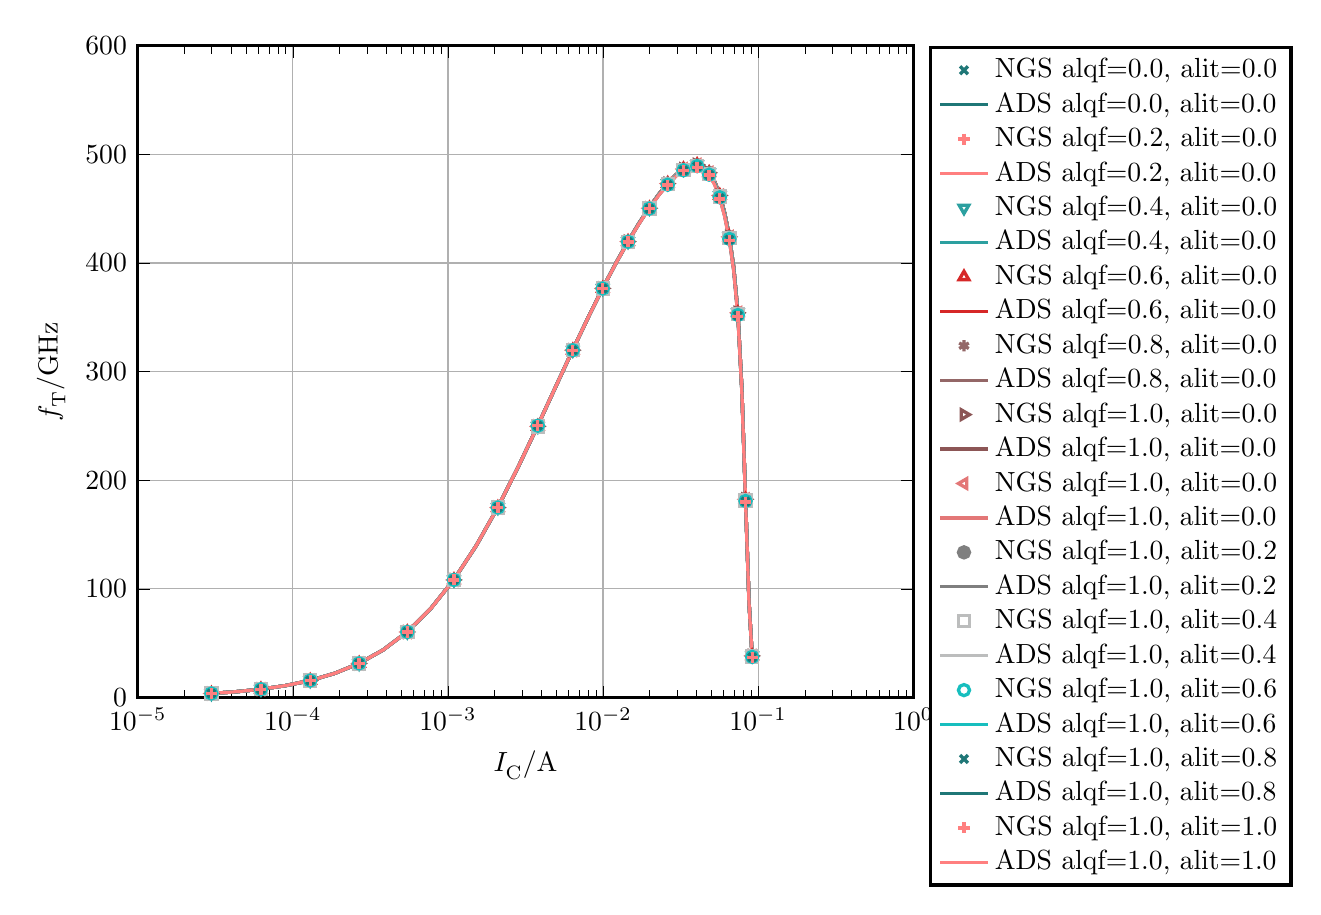
\begin{tikzpicture}[font=\normalsize]
\pgfplotsset{every axis/.append style={very thick}},
\definecolor{color0}{rgb}{0.12157, 0.46667, 0.46667}
\definecolor{color1}{rgb}{1.00000, 0.49804, 0.49804}
\definecolor{color2}{rgb}{0.17255, 0.62745, 0.62745}
\definecolor{color3}{rgb}{0.83922, 0.15294, 0.15294}
\definecolor{color4}{rgb}{0.58039, 0.40392, 0.40392}
\definecolor{color5}{rgb}{0.54902, 0.33725, 0.33725}
\definecolor{color6}{rgb}{0.89020, 0.46667, 0.46667}
\definecolor{color7}{rgb}{0.49804, 0.49804, 0.49804}
\definecolor{color8}{rgb}{0.73725, 0.74118, 0.74118}
\definecolor{color9}{rgb}{0.09020, 0.74510, 0.74510}

\begin{axis}[
width=4.5in,
xlabel={$I_{\mathrm{C}}^{}/\si{\ampere}$},
ylabel={$f_{\mathrm{T}}^{}/\si{\giga\hertz}$},
xmode=log,
xmin=1e-05,
xmax=1,
restrict x to domain=-5:0,
log basis x=10,
ymin=0,
ymax=600,
restrict y to domain=0:600,
log basis y=10,
xmajorgrids,
enlargelimits=false,
scaled ticks=false,
ymajorgrids,
x tick style={color=black},
y tick style={color=black},
x grid style={white!69.01960784313725!black},
y grid style={white!69.01960784313725!black},
/tikz/mark repeat=2,
legend style={at={(1.02,1.00)}, anchor=north west,legend cell align=left, align=left},
]
\addplot [color=color0, only marks, mark=x, mark options={solid}, mark phase=0, ]
  table[row sep=crcr, x expr=\thisrowno{0}*1.000000e+00, y expr=\thisrowno{1}*1.000000e-09]{
2.98396e-05 3.7103e+09\\
4.31177e-05 5.3303e+09\\
6.225e-05 7.65253e+09\\
8.97943e-05 1.09417e+10\\
0.000129401 1.56223e+10\\
0.000186243 2.21828e+10\\
0.000267564 3.13818e+10\\
0.000383354 4.38786e+10\\
0.000547084 6.03275e+10\\
0.000776382 8.18374e+10\\
0.00109339 1.08568e+11\\
0.00152451 1.40064e+11\\
0.00209913 1.74873e+11\\
0.00284735 2.1259e+11\\
0.00379703 2.50195e+11\\
0.00497087 2.8593e+11\\
0.00638447 3.19761e+11\\
0.00804567 3.49817e+11\\
0.0099552 3.76643e+11\\
0.012108 3.99286e+11\\
0.0144948 4.19769e+11\\
0.0171038 4.36956e+11\\
0.0199213 4.51143e+11\\
0.0229333 4.63334e+11\\
0.0261255 4.72548e+11\\
0.0294841 4.8106e+11\\
0.0329955 4.85948e+11\\
0.0366471 4.90655e+11\\
0.0404269 4.91097e+11\\
0.0443236 4.88864e+11\\
0.0483264 4.83167e+11\\
0.0524253 4.74985e+11\\
0.0566106 4.62728e+11\\
0.060873 4.45371e+11\\
0.0652035 4.24128e+11\\
0.0695925 3.96258e+11\\
0.0740296 3.54461e+11\\
0.0784992 2.84981e+11\\
0.08297 1.82551e+11\\
0.0873655 8.81619e+10\\
0.0915303 3.83321e+10\\
};
\addlegendentry{NGS alqf=0.0, alit=0.0}
\addplot [color=color0, solid,  mark phase=0, ]
  table[row sep=crcr, x expr=\thisrowno{0}*1.000000e+00, y expr=\thisrowno{1}*1.000000e-09]{
2.98384e-05 3.70997e+09\\
4.31161e-05 5.33215e+09\\
6.22476e-05 7.65375e+09\\
8.97908e-05 1.09652e+10\\
0.000129396 1.56617e+10\\
0.000186236 2.22643e+10\\
0.000267554 3.1429e+10\\
0.000383339 4.39242e+10\\
0.000547063 6.05531e+10\\
0.000776351 8.19942e+10\\
0.00109335 1.08568e+11\\
0.00152446 1.39988e+11\\
0.00209905 1.75236e+11\\
0.00284725 2.1267e+11\\
0.0037969 2.50381e+11\\
0.00497072 2.86632e+11\\
0.00638428 3.20174e+11\\
0.00804546 3.50328e+11\\
0.00995495 3.76898e+11\\
0.0121077 4.00002e+11\\
0.0144945 4.19916e+11\\
0.0171034 4.36961e+11\\
0.019921 4.51429e+11\\
0.0229329 4.63552e+11\\
0.0261251 4.73476e+11\\
0.0294836 4.81254e+11\\
0.032995 4.86848e+11\\
0.0366466 4.90127e+11\\
0.0404264 4.90879e+11\\
0.0443231 4.88826e+11\\
0.0483259 4.83647e+11\\
0.0524248 4.75012e+11\\
0.0566101 4.62595e+11\\
0.0608725 4.46031e+11\\
0.0652029 4.24618e+11\\
0.069592 3.96247e+11\\
0.074029 3.54454e+11\\
0.0784986 2.85095e+11\\
0.0829694 1.82583e+11\\
0.0873649 8.81736e+10\\
0.0915297 3.83405e+10\\
};
\addlegendentry{ADS alqf=0.0, alit=0.0}
\addplot [color=color1, only marks, mark=+, mark options={solid}, mark phase=0, ]
  table[row sep=crcr, x expr=\thisrowno{0}*1.000000e+00, y expr=\thisrowno{1}*1.000000e-09]{
2.98396e-05 3.69841e+09\\
4.31177e-05 5.3303e+09\\
6.225e-05 7.62815e+09\\
8.97943e-05 1.09417e+10\\
0.000129401 1.56223e+10\\
0.000186243 2.21828e+10\\
0.000267564 3.13818e+10\\
0.000383354 4.38786e+10\\
0.000547084 6.03275e+10\\
0.000776382 8.18374e+10\\
0.00109339 1.08264e+11\\
0.00152451 1.39689e+11\\
0.00209913 1.74873e+11\\
0.00284735 2.1208e+11\\
0.00379703 2.49632e+11\\
0.00497087 2.86535e+11\\
0.00638447 3.19761e+11\\
0.00804567 3.49817e+11\\
0.0099552 3.76643e+11\\
0.012108 3.99285e+11\\
0.0144948 4.19768e+11\\
0.0171038 4.36286e+11\\
0.0199213 4.50478e+11\\
0.0229333 4.63333e+11\\
0.0261255 4.73198e+11\\
0.0294841 4.80418e+11\\
0.0329955 4.86576e+11\\
0.0366471 4.89422e+11\\
0.0404269 4.90498e+11\\
0.0443236 4.88287e+11\\
0.0483264 4.83166e+11\\
0.0524253 4.74984e+11\\
0.0566106 4.62244e+11\\
0.060873 4.4581e+11\\
0.0652035 4.24126e+11\\
0.0695925 3.95917e+11\\
0.0740296 3.54191e+11\\
0.0784992 2.84978e+11\\
0.08297 1.82546e+11\\
0.0873655 8.81528e+10\\
0.0915303 3.8334e+10\\
};
\addlegendentry{NGS alqf=0.2, alit=0.0}
\addplot [color=color1, solid,  mark phase=0, ]
  table[row sep=crcr, x expr=\thisrowno{0}*1.000000e+00, y expr=\thisrowno{1}*1.000000e-09]{
2.98384e-05 3.70997e+09\\
4.31161e-05 5.33215e+09\\
6.22476e-05 7.65375e+09\\
8.97908e-05 1.09652e+10\\
0.000129396 1.56617e+10\\
0.000186236 2.22643e+10\\
0.000267554 3.1429e+10\\
0.000383339 4.39242e+10\\
0.000547063 6.05531e+10\\
0.000776351 8.19942e+10\\
0.00109335 1.08568e+11\\
0.00152446 1.39988e+11\\
0.00209905 1.75236e+11\\
0.00284725 2.1267e+11\\
0.0037969 2.50381e+11\\
0.00497072 2.86632e+11\\
0.00638428 3.20174e+11\\
0.00804546 3.50328e+11\\
0.00995495 3.76898e+11\\
0.0121077 4.00002e+11\\
0.0144945 4.19916e+11\\
0.0171034 4.36961e+11\\
0.019921 4.51429e+11\\
0.0229329 4.63552e+11\\
0.0261251 4.73476e+11\\
0.0294836 4.81254e+11\\
0.032995 4.86848e+11\\
0.0366466 4.90127e+11\\
0.0404264 4.90879e+11\\
0.0443231 4.88826e+11\\
0.0483259 4.83647e+11\\
0.0524248 4.75012e+11\\
0.0566101 4.62595e+11\\
0.0608725 4.46031e+11\\
0.0652029 4.24618e+11\\
0.069592 3.96246e+11\\
0.074029 3.54454e+11\\
0.0784986 2.85095e+11\\
0.0829694 1.82583e+11\\
0.0873649 8.81736e+10\\
0.0915297 3.83406e+10\\
};
\addlegendentry{ADS alqf=0.2, alit=0.0}
\addplot [color=color2, only marks, mark=triangle, mark options={solid, rotate=180}, mark phase=0, ]
  table[row sep=crcr, x expr=\thisrowno{0}*1.000000e+00, y expr=\thisrowno{1}*1.000000e-09]{
2.98396e-05 3.69841e+09\\
4.31177e-05 5.3303e+09\\
6.225e-05 7.62815e+09\\
8.97943e-05 1.09417e+10\\
0.000129401 1.56223e+10\\
0.000186243 2.21828e+10\\
0.000267564 3.13818e+10\\
0.000383354 4.38786e+10\\
0.000547084 6.03275e+10\\
0.000776382 8.18374e+10\\
0.00109339 1.08264e+11\\
0.00152451 1.39689e+11\\
0.00209913 1.74873e+11\\
0.00284735 2.1208e+11\\
0.00379703 2.49632e+11\\
0.00497087 2.86534e+11\\
0.00638447 3.1976e+11\\
0.00804567 3.49817e+11\\
0.0099552 3.76642e+11\\
0.012108 3.99285e+11\\
0.0144948 4.19768e+11\\
0.0171038 4.36285e+11\\
0.0199213 4.50478e+11\\
0.0229333 4.63332e+11\\
0.0261255 4.73197e+11\\
0.0294841 4.80417e+11\\
0.0329955 4.86575e+11\\
0.0366471 4.89421e+11\\
0.0404269 4.90497e+11\\
0.0443236 4.88286e+11\\
0.0483264 4.83164e+11\\
0.0524253 4.74982e+11\\
0.0566106 4.62243e+11\\
0.060873 4.45808e+11\\
0.0652035 4.24125e+11\\
0.0695925 3.95915e+11\\
0.0740296 3.54189e+11\\
0.0784992 2.84975e+11\\
0.08297 1.82541e+11\\
0.0873655 8.81431e+10\\
0.0915303 3.83361e+10\\
};
\addlegendentry{NGS alqf=0.4, alit=0.0}
\addplot [color=color2, solid,  mark phase=0, ]
  table[row sep=crcr, x expr=\thisrowno{0}*1.000000e+00, y expr=\thisrowno{1}*1.000000e-09]{
2.98384e-05 3.70997e+09\\
4.31161e-05 5.33215e+09\\
6.22476e-05 7.65375e+09\\
8.97908e-05 1.09652e+10\\
0.000129396 1.56617e+10\\
0.000186236 2.22643e+10\\
0.000267554 3.1429e+10\\
0.000383339 4.39242e+10\\
0.000547063 6.05531e+10\\
0.000776351 8.19942e+10\\
0.00109335 1.08568e+11\\
0.00152446 1.39988e+11\\
0.00209905 1.75236e+11\\
0.00284725 2.1267e+11\\
0.0037969 2.50381e+11\\
0.00497072 2.86632e+11\\
0.00638428 3.20174e+11\\
0.00804546 3.50328e+11\\
0.00995495 3.76898e+11\\
0.0121077 4.00002e+11\\
0.0144945 4.19916e+11\\
0.0171034 4.3696e+11\\
0.019921 4.51429e+11\\
0.0229329 4.63552e+11\\
0.0261251 4.73476e+11\\
0.0294836 4.81254e+11\\
0.032995 4.86848e+11\\
0.0366466 4.90127e+11\\
0.0404264 4.90879e+11\\
0.0443231 4.88826e+11\\
0.0483259 4.83647e+11\\
0.0524248 4.75012e+11\\
0.0566101 4.62595e+11\\
0.0608725 4.46031e+11\\
0.0652029 4.24618e+11\\
0.069592 3.96246e+11\\
0.074029 3.54454e+11\\
0.0784986 2.85095e+11\\
0.0829694 1.82583e+11\\
0.0873649 8.81741e+10\\
0.0915297 3.83421e+10\\
};
\addlegendentry{ADS alqf=0.4, alit=0.0}
\addplot [color=color3, only marks, mark=triangle, mark options={solid, rotate=0}, mark phase=0, ]
  table[row sep=crcr, x expr=\thisrowno{0}*1.000000e+00, y expr=\thisrowno{1}*1.000000e-09]{
2.98396e-05 3.69841e+09\\
4.31177e-05 5.3303e+09\\
6.225e-05 7.62815e+09\\
8.97943e-05 1.09417e+10\\
0.000129401 1.56223e+10\\
0.000186243 2.21828e+10\\
0.000267564 3.13818e+10\\
0.000383354 4.38786e+10\\
0.000547084 6.03275e+10\\
0.000776382 8.18374e+10\\
0.00109339 1.08264e+11\\
0.00152451 1.39689e+11\\
0.00209913 1.74873e+11\\
0.00284735 2.1208e+11\\
0.00379703 2.49632e+11\\
0.00497087 2.86534e+11\\
0.00638447 3.1976e+11\\
0.00804567 3.49816e+11\\
0.0099552 3.76642e+11\\
0.012108 3.99284e+11\\
0.0144948 4.19767e+11\\
0.0171038 4.36284e+11\\
0.0199213 4.50477e+11\\
0.0229333 4.63331e+11\\
0.0261255 4.73196e+11\\
0.0294841 4.80416e+11\\
0.0329955 4.86574e+11\\
0.0366471 4.8942e+11\\
0.0404269 4.90496e+11\\
0.0443236 4.88284e+11\\
0.0483264 4.83163e+11\\
0.0524253 4.74981e+11\\
0.0566106 4.62241e+11\\
0.060873 4.45807e+11\\
0.0652035 4.24123e+11\\
0.0695925 3.95913e+11\\
0.0740296 3.54186e+11\\
0.0784992 2.84973e+11\\
0.08297 1.82537e+11\\
0.0873655 8.81506e+10\\
0.0915303 3.83384e+10\\
};
\addlegendentry{NGS alqf=0.6, alit=0.0}
\addplot [color=color3, solid,  mark phase=0, ]
  table[row sep=crcr, x expr=\thisrowno{0}*1.000000e+00, y expr=\thisrowno{1}*1.000000e-09]{
2.98384e-05 3.70997e+09\\
4.31161e-05 5.33215e+09\\
6.22476e-05 7.65375e+09\\
8.97908e-05 1.09652e+10\\
0.000129396 1.56617e+10\\
0.000186236 2.22643e+10\\
0.000267554 3.1429e+10\\
0.000383339 4.39242e+10\\
0.000547063 6.05531e+10\\
0.000776351 8.19942e+10\\
0.00109335 1.08568e+11\\
0.00152446 1.39988e+11\\
0.00209905 1.75236e+11\\
0.00284725 2.1267e+11\\
0.0037969 2.50381e+11\\
0.00497072 2.86632e+11\\
0.00638428 3.20174e+11\\
0.00804546 3.50328e+11\\
0.00995495 3.76898e+11\\
0.0121077 4.00002e+11\\
0.0144945 4.19916e+11\\
0.0171034 4.3696e+11\\
0.019921 4.51429e+11\\
0.0229329 4.63552e+11\\
0.0261251 4.73476e+11\\
0.0294836 4.81254e+11\\
0.032995 4.86848e+11\\
0.0366466 4.90127e+11\\
0.0404264 4.90879e+11\\
0.0443231 4.88826e+11\\
0.0483259 4.83647e+11\\
0.0524248 4.75012e+11\\
0.0566101 4.62595e+11\\
0.0608725 4.46031e+11\\
0.0652029 4.24618e+11\\
0.069592 3.96247e+11\\
0.074029 3.54454e+11\\
0.0784986 2.85096e+11\\
0.0829694 1.82583e+11\\
0.0873649 8.81752e+10\\
0.0915297 3.83449e+10\\
};
\addlegendentry{ADS alqf=0.6, alit=0.0}
\addplot [color=color4, only marks, mark=asterisk, mark options={solid}, mark phase=0, ]
  table[row sep=crcr, x expr=\thisrowno{0}*1.000000e+00, y expr=\thisrowno{1}*1.000000e-09]{
2.98396e-05 3.69841e+09\\
4.31177e-05 5.3303e+09\\
6.225e-05 7.62815e+09\\
8.97943e-05 1.09417e+10\\
0.000129401 1.56223e+10\\
0.000186243 2.21828e+10\\
0.000267564 3.13818e+10\\
0.000383354 4.38786e+10\\
0.000547084 6.03275e+10\\
0.000776382 8.18373e+10\\
0.00109339 1.08264e+11\\
0.00152451 1.39689e+11\\
0.00209913 1.74873e+11\\
0.00284735 2.1208e+11\\
0.00379703 2.49632e+11\\
0.00497087 2.86534e+11\\
0.00638447 3.1976e+11\\
0.00804567 3.49816e+11\\
0.0099552 3.76641e+11\\
0.012108 3.99284e+11\\
0.0144948 4.19767e+11\\
0.0171038 4.36284e+11\\
0.0199213 4.50476e+11\\
0.0229333 4.63331e+11\\
0.0261255 4.73195e+11\\
0.0294841 4.80415e+11\\
0.0329955 4.86573e+11\\
0.0366471 4.89419e+11\\
0.0404269 4.90495e+11\\
0.0443236 4.88283e+11\\
0.0483264 4.83162e+11\\
0.0524253 4.7498e+11\\
0.0566106 4.6224e+11\\
0.060873 4.45805e+11\\
0.0652035 4.24121e+11\\
0.0695925 3.95912e+11\\
0.0740296 3.54184e+11\\
0.0784992 2.8497e+11\\
0.08297 1.82532e+11\\
0.0873655 8.81582e+10\\
0.0915303 3.83411e+10\\
};
\addlegendentry{NGS alqf=0.8, alit=0.0}
\addplot [color=color4, solid,  mark phase=0, ]
  table[row sep=crcr, x expr=\thisrowno{0}*1.000000e+00, y expr=\thisrowno{1}*1.000000e-09]{
2.98384e-05 3.70997e+09\\
4.31161e-05 5.33215e+09\\
6.22476e-05 7.65375e+09\\
8.97908e-05 1.09652e+10\\
0.000129396 1.56617e+10\\
0.000186236 2.22643e+10\\
0.000267554 3.1429e+10\\
0.000383339 4.39242e+10\\
0.000547063 6.05531e+10\\
0.000776351 8.19942e+10\\
0.00109335 1.08568e+11\\
0.00152446 1.39988e+11\\
0.00209905 1.75236e+11\\
0.00284725 2.1267e+11\\
0.0037969 2.50381e+11\\
0.00497072 2.86632e+11\\
0.00638428 3.20174e+11\\
0.00804546 3.50328e+11\\
0.00995495 3.76898e+11\\
0.0121077 4.00002e+11\\
0.0144945 4.19916e+11\\
0.0171034 4.36961e+11\\
0.019921 4.51429e+11\\
0.0229329 4.63552e+11\\
0.0261251 4.73476e+11\\
0.0294836 4.81254e+11\\
0.032995 4.86848e+11\\
0.0366466 4.90127e+11\\
0.0404264 4.90879e+11\\
0.0443231 4.88826e+11\\
0.0483259 4.83647e+11\\
0.0524248 4.75012e+11\\
0.0566101 4.62595e+11\\
0.0608725 4.46031e+11\\
0.0652029 4.24618e+11\\
0.069592 3.96247e+11\\
0.074029 3.54454e+11\\
0.0784986 2.85096e+11\\
0.0829694 1.82584e+11\\
0.0873649 8.81768e+10\\
0.0915297 3.83491e+10\\
};
\addlegendentry{ADS alqf=0.8, alit=0.0}
\addplot [color=color5, only marks, mark=triangle, mark options={solid, rotate=270}, mark phase=0, ]
  table[row sep=crcr, x expr=\thisrowno{0}*1.000000e+00, y expr=\thisrowno{1}*1.000000e-09]{
2.98396e-05 3.69841e+09\\
4.31177e-05 5.3303e+09\\
6.225e-05 7.62815e+09\\
8.97943e-05 1.09417e+10\\
0.000129401 1.56223e+10\\
0.000186243 2.21828e+10\\
0.000267564 3.13818e+10\\
0.000383354 4.38786e+10\\
0.000547084 6.03275e+10\\
0.000776382 8.18373e+10\\
0.00109339 1.08264e+11\\
0.00152451 1.39689e+11\\
0.00209913 1.74873e+11\\
0.00284735 2.1208e+11\\
0.00379703 2.49632e+11\\
0.00497087 2.86534e+11\\
0.00638447 3.1976e+11\\
0.00804567 3.49816e+11\\
0.0099552 3.76641e+11\\
0.012108 3.99283e+11\\
0.0144948 4.19766e+11\\
0.0171038 4.36283e+11\\
0.0199213 4.50476e+11\\
0.0229333 4.6333e+11\\
0.0261255 4.73194e+11\\
0.0294841 4.80414e+11\\
0.0329955 4.86572e+11\\
0.0366471 4.89418e+11\\
0.0404269 4.90494e+11\\
0.0443236 4.88282e+11\\
0.0483264 4.83161e+11\\
0.0524253 4.74978e+11\\
0.0566106 4.62239e+11\\
0.060873 4.45804e+11\\
0.0652035 4.2412e+11\\
0.0695925 3.9591e+11\\
0.0740296 3.54182e+11\\
0.0784992 2.84967e+11\\
0.08297 1.82527e+11\\
0.0873655 8.81659e+10\\
0.0915303 3.83475e+10\\
};
\addlegendentry{NGS alqf=1.0, alit=0.0}
\addplot [color=color5, solid,  mark phase=0, ]
  table[row sep=crcr, x expr=\thisrowno{0}*1.000000e+00, y expr=\thisrowno{1}*1.000000e-09]{
2.98384e-05 3.70997e+09\\
4.31161e-05 5.33215e+09\\
6.22476e-05 7.65375e+09\\
8.97908e-05 1.09652e+10\\
0.000129396 1.56617e+10\\
0.000186236 2.22643e+10\\
0.000267554 3.1429e+10\\
0.000383339 4.39242e+10\\
0.000547063 6.05531e+10\\
0.000776351 8.19942e+10\\
0.00109335 1.08568e+11\\
0.00152446 1.39988e+11\\
0.00209905 1.75236e+11\\
0.00284725 2.1267e+11\\
0.0037969 2.50381e+11\\
0.00497072 2.86632e+11\\
0.00638428 3.20174e+11\\
0.00804546 3.50328e+11\\
0.00995495 3.76898e+11\\
0.0121077 4.00002e+11\\
0.0144945 4.19916e+11\\
0.0171034 4.36961e+11\\
0.019921 4.51429e+11\\
0.0229329 4.63552e+11\\
0.0261251 4.73476e+11\\
0.0294836 4.81254e+11\\
0.032995 4.86848e+11\\
0.0366466 4.90127e+11\\
0.0404264 4.90879e+11\\
0.0443231 4.88826e+11\\
0.0483259 4.83648e+11\\
0.0524248 4.75012e+11\\
0.0566101 4.62595e+11\\
0.0608725 4.46031e+11\\
0.0652029 4.24618e+11\\
0.069592 3.96247e+11\\
0.074029 3.54454e+11\\
0.0784986 2.85096e+11\\
0.0829694 1.82585e+11\\
0.0873649 8.81791e+10\\
0.0915297 3.83546e+10\\
};
\addlegendentry{ADS alqf=1.0, alit=0.0}
\addplot [color=color6, only marks, mark=triangle, mark options={solid, rotate=90}, mark phase=0, ]
  table[row sep=crcr, x expr=\thisrowno{0}*1.000000e+00, y expr=\thisrowno{1}*1.000000e-09]{
2.98396e-05 3.69841e+09\\
4.31177e-05 5.3303e+09\\
6.225e-05 7.62815e+09\\
8.97943e-05 1.09417e+10\\
0.000129401 1.56223e+10\\
0.000186243 2.21828e+10\\
0.000267564 3.13818e+10\\
0.000383354 4.38786e+10\\
0.000547084 6.03275e+10\\
0.000776382 8.18373e+10\\
0.00109339 1.08264e+11\\
0.00152451 1.39689e+11\\
0.00209913 1.74873e+11\\
0.00284735 2.1208e+11\\
0.00379703 2.49632e+11\\
0.00497087 2.86534e+11\\
0.00638447 3.1976e+11\\
0.00804567 3.49816e+11\\
0.0099552 3.76641e+11\\
0.012108 3.99283e+11\\
0.0144948 4.19766e+11\\
0.0171038 4.36283e+11\\
0.0199213 4.50476e+11\\
0.0229333 4.6333e+11\\
0.0261255 4.73194e+11\\
0.0294841 4.80414e+11\\
0.0329955 4.86572e+11\\
0.0366471 4.89418e+11\\
0.0404269 4.90494e+11\\
0.0443236 4.88282e+11\\
0.0483264 4.83161e+11\\
0.0524253 4.74978e+11\\
0.0566106 4.62239e+11\\
0.060873 4.45804e+11\\
0.0652035 4.2412e+11\\
0.0695925 3.9591e+11\\
0.0740296 3.54182e+11\\
0.0784992 2.84967e+11\\
0.08297 1.82527e+11\\
0.0873655 8.81659e+10\\
0.0915303 3.83475e+10\\
};
\addlegendentry{NGS alqf=1.0, alit=0.0}
\addplot [color=color6, solid,  mark phase=0, ]
  table[row sep=crcr, x expr=\thisrowno{0}*1.000000e+00, y expr=\thisrowno{1}*1.000000e-09]{
2.98384e-05 3.70997e+09\\
4.31161e-05 5.33215e+09\\
6.22476e-05 7.65375e+09\\
8.97908e-05 1.09652e+10\\
0.000129396 1.56617e+10\\
0.000186236 2.22643e+10\\
0.000267554 3.1429e+10\\
0.000383339 4.39242e+10\\
0.000547063 6.05531e+10\\
0.000776351 8.19942e+10\\
0.00109335 1.08568e+11\\
0.00152446 1.39988e+11\\
0.00209905 1.75236e+11\\
0.00284725 2.1267e+11\\
0.0037969 2.50381e+11\\
0.00497072 2.86632e+11\\
0.00638428 3.20174e+11\\
0.00804546 3.50328e+11\\
0.00995495 3.76898e+11\\
0.0121077 4.00002e+11\\
0.0144945 4.19916e+11\\
0.0171034 4.36961e+11\\
0.019921 4.51429e+11\\
0.0229329 4.63552e+11\\
0.0261251 4.73476e+11\\
0.0294836 4.81254e+11\\
0.032995 4.86848e+11\\
0.0366466 4.90127e+11\\
0.0404264 4.90879e+11\\
0.0443231 4.88826e+11\\
0.0483259 4.83648e+11\\
0.0524248 4.75012e+11\\
0.0566101 4.62595e+11\\
0.0608725 4.46031e+11\\
0.0652029 4.24618e+11\\
0.069592 3.96247e+11\\
0.074029 3.54454e+11\\
0.0784986 2.85096e+11\\
0.0829694 1.82585e+11\\
0.0873649 8.81791e+10\\
0.0915297 3.83546e+10\\
};
\addlegendentry{ADS alqf=1.0, alit=0.0}
\addplot [color=color7, only marks, mark=*, mark options={solid, fill}, mark phase=0, ]
  table[row sep=crcr, x expr=\thisrowno{0}*1.000000e+00, y expr=\thisrowno{1}*1.000000e-09]{
2.98396e-05 3.69846e+09\\
4.31177e-05 5.33037e+09\\
6.225e-05 7.62826e+09\\
8.97943e-05 1.09419e+10\\
0.000129401 1.56226e+10\\
0.000186243 2.21834e+10\\
0.000267564 3.13828e+10\\
0.000383354 4.38804e+10\\
0.000547084 6.03306e+10\\
0.000776382 8.18423e+10\\
0.00109339 1.08272e+11\\
0.00152451 1.39699e+11\\
0.00209913 1.74887e+11\\
0.00284735 2.12095e+11\\
0.00379703 2.49646e+11\\
0.00497087 2.86543e+11\\
0.00638447 3.1976e+11\\
0.00804567 3.49802e+11\\
0.0099552 3.76611e+11\\
0.012108 3.99235e+11\\
0.0144948 4.19697e+11\\
0.0171038 4.36193e+11\\
0.0199213 4.50364e+11\\
0.0229333 4.63198e+11\\
0.0261255 4.73044e+11\\
0.0294841 4.80246e+11\\
0.0329955 4.85759e+11\\
0.0366471 4.8922e+11\\
0.0404269 4.89686e+11\\
0.0443236 4.88059e+11\\
0.0483264 4.82929e+11\\
0.0524253 4.7422e+11\\
0.0566106 4.61512e+11\\
0.060873 4.45115e+11\\
0.0652035 4.23871e+11\\
0.0695925 3.95326e+11\\
0.0740296 3.53677e+11\\
0.0784992 2.84406e+11\\
0.08297 1.81994e+11\\
0.0873655 8.77714e+10\\
0.0915303 3.80377e+10\\
};
\addlegendentry{NGS alqf=1.0, alit=0.2}
\addplot [color=color7, solid,  mark phase=0, ]
  table[row sep=crcr, x expr=\thisrowno{0}*1.000000e+00, y expr=\thisrowno{1}*1.000000e-09]{
2.98384e-05 3.71002e+09\\
4.31161e-05 5.33222e+09\\
6.22476e-05 7.65386e+09\\
8.97908e-05 1.09654e+10\\
0.000129396 1.5662e+10\\
0.000186236 2.22649e+10\\
0.000267554 3.143e+10\\
0.000383339 4.39261e+10\\
0.000547063 6.05563e+10\\
0.000776351 8.19996e+10\\
0.00109335 1.08576e+11\\
0.00152446 1.40001e+11\\
0.00209905 1.75253e+11\\
0.00284725 2.12691e+11\\
0.0037969 2.50403e+11\\
0.00497072 2.86652e+11\\
0.00638428 3.20187e+11\\
0.00804546 3.50328e+11\\
0.00995495 3.76879e+11\\
0.0121077 3.99959e+11\\
0.0144945 4.19842e+11\\
0.0171034 4.36852e+11\\
0.019921 4.51281e+11\\
0.0229329 4.63361e+11\\
0.0261251 4.7324e+11\\
0.0294836 4.80971e+11\\
0.032995 4.86515e+11\\
0.0366466 4.89744e+11\\
0.0404264 4.90445e+11\\
0.0443231 4.88342e+11\\
0.0483259 4.83116e+11\\
0.0524248 4.74436e+11\\
0.0566101 4.61978e+11\\
0.0608725 4.45378e+11\\
0.0652029 4.23937e+11\\
0.069592 3.9555e+11\\
0.074029 3.53763e+11\\
0.0784986 2.84455e+11\\
0.0829694 1.82061e+11\\
0.0873649 8.77896e+10\\
0.0915297 3.80449e+10\\
};
\addlegendentry{ADS alqf=1.0, alit=0.2}
\addplot [color=color8, only marks, mark=square, mark options={solid}, mark phase=0, ]
  table[row sep=crcr, x expr=\thisrowno{0}*1.000000e+00, y expr=\thisrowno{1}*1.000000e-09]{
2.98396e-05 3.69851e+09\\
4.31177e-05 5.33044e+09\\
6.225e-05 7.62837e+09\\
8.97943e-05 1.09421e+10\\
0.000129401 1.56229e+10\\
0.000186243 2.2184e+10\\
0.000267564 3.13838e+10\\
0.000383354 4.38822e+10\\
0.000547084 6.03336e+10\\
0.000776382 8.18474e+10\\
0.00109339 1.08279e+11\\
0.00152451 1.3971e+11\\
0.00209913 1.749e+11\\
0.00284735 2.12111e+11\\
0.00379703 2.4966e+11\\
0.00497087 2.86552e+11\\
0.00638447 3.1976e+11\\
0.00804567 3.49789e+11\\
0.0099552 3.76581e+11\\
0.012108 3.99186e+11\\
0.0144948 4.19627e+11\\
0.0171038 4.36102e+11\\
0.0199213 4.50253e+11\\
0.0229333 4.63067e+11\\
0.0261255 4.72893e+11\\
0.0294841 4.80078e+11\\
0.0329955 4.85575e+11\\
0.0366471 4.89021e+11\\
0.0404269 4.89474e+11\\
0.0443236 4.87837e+11\\
0.0483264 4.82149e+11\\
0.0524253 4.73465e+11\\
0.0566106 4.61268e+11\\
0.060873 4.44429e+11\\
0.0652035 4.22839e+11\\
0.0695925 3.94407e+11\\
0.0740296 3.52907e+11\\
0.0784992 2.83676e+11\\
0.08297 1.81465e+11\\
0.0873655 8.73806e+10\\
0.0915303 3.77333e+10\\
};
\addlegendentry{NGS alqf=1.0, alit=0.4}
\addplot [color=color8, solid,  mark phase=0, ]
  table[row sep=crcr, x expr=\thisrowno{0}*1.000000e+00, y expr=\thisrowno{1}*1.000000e-09]{
2.98384e-05 3.71008e+09\\
4.31161e-05 5.3323e+09\\
6.22476e-05 7.65397e+09\\
8.97908e-05 1.09655e+10\\
0.000129396 1.56623e+10\\
0.000186236 2.22655e+10\\
0.000267554 3.1431e+10\\
0.000383339 4.3928e+10\\
0.000547063 6.05595e+10\\
0.000776351 8.2005e+10\\
0.00109335 1.08585e+11\\
0.00152446 1.40013e+11\\
0.00209905 1.7527e+11\\
0.00284725 2.12711e+11\\
0.0037969 2.50425e+11\\
0.00497072 2.86672e+11\\
0.00638428 3.20199e+11\\
0.00804546 3.50328e+11\\
0.00995495 3.7686e+11\\
0.0121077 3.99915e+11\\
0.0144945 4.19768e+11\\
0.0171034 4.36743e+11\\
0.019921 4.51133e+11\\
0.0229329 4.63171e+11\\
0.0261251 4.73004e+11\\
0.0294836 4.80687e+11\\
0.032995 4.86182e+11\\
0.0366466 4.89361e+11\\
0.0404264 4.90012e+11\\
0.0443231 4.8786e+11\\
0.0483259 4.82586e+11\\
0.0524248 4.73861e+11\\
0.0566101 4.61362e+11\\
0.0608725 4.44727e+11\\
0.0652029 4.23258e+11\\
0.069592 3.94855e+11\\
0.074029 3.53073e+11\\
0.0784986 2.83817e+11\\
0.0829694 1.81541e+11\\
0.0873649 8.74038e+10\\
0.0915297 3.77405e+10\\
};
\addlegendentry{ADS alqf=1.0, alit=0.4}
\addplot [color=color9, only marks, mark=o, mark options={solid, fill}, mark phase=0, ]
  table[row sep=crcr, x expr=\thisrowno{0}*1.000000e+00, y expr=\thisrowno{1}*1.000000e-09]{
2.98396e-05 3.69857e+09\\
4.31177e-05 5.33052e+09\\
6.225e-05 7.62848e+09\\
8.97943e-05 1.09422e+10\\
0.000129401 1.56233e+10\\
0.000186243 2.21845e+10\\
0.000267564 3.13848e+10\\
0.000383354 4.3884e+10\\
0.000547084 6.03367e+10\\
0.000776382 8.18524e+10\\
0.00109339 1.08287e+11\\
0.00152451 1.39721e+11\\
0.00209913 1.74914e+11\\
0.00284735 2.12126e+11\\
0.00379703 2.50237e+11\\
0.00497087 2.86562e+11\\
0.00638447 3.1976e+11\\
0.00804567 3.49776e+11\\
0.0099552 3.76551e+11\\
0.012108 3.99137e+11\\
0.0144948 4.19558e+11\\
0.0171038 4.36012e+11\\
0.0199213 4.50142e+11\\
0.0229333 4.62935e+11\\
0.0261255 4.72094e+11\\
0.0294841 4.79911e+11\\
0.0329955 4.85391e+11\\
0.0366471 4.88211e+11\\
0.0404269 4.89263e+11\\
0.0443236 4.87041e+11\\
0.0483264 4.81372e+11\\
0.0524253 4.72711e+11\\
0.0566106 4.60545e+11\\
0.060873 4.43745e+11\\
0.0652035 4.22202e+11\\
0.0695925 3.94163e+11\\
0.0740296 3.52139e+11\\
0.0784992 2.8312e+11\\
0.08297 1.80938e+11\\
0.0873655 8.70102e+10\\
0.0915303 3.74343e+10\\
};
\addlegendentry{NGS alqf=1.0, alit=0.6}
\addplot [color=color9, solid,  mark phase=0, ]
  table[row sep=crcr, x expr=\thisrowno{0}*1.000000e+00, y expr=\thisrowno{1}*1.000000e-09]{
2.98384e-05 3.71013e+09\\
4.31161e-05 5.33237e+09\\
6.22476e-05 7.65408e+09\\
8.97908e-05 1.09657e+10\\
0.000129396 1.56626e+10\\
0.000186236 2.2266e+10\\
0.000267554 3.14321e+10\\
0.000383339 4.39298e+10\\
0.000547063 6.05628e+10\\
0.000776351 8.20104e+10\\
0.00109335 1.08593e+11\\
0.00152446 1.40026e+11\\
0.00209905 1.75287e+11\\
0.00284725 2.12732e+11\\
0.0037969 2.50447e+11\\
0.00497072 2.86692e+11\\
0.00638428 3.20212e+11\\
0.00804546 3.50328e+11\\
0.00995495 3.76841e+11\\
0.0121077 3.99871e+11\\
0.0144945 4.19694e+11\\
0.0171034 4.36634e+11\\
0.019921 4.50985e+11\\
0.0229329 4.6298e+11\\
0.0261251 4.72768e+11\\
0.0294836 4.80404e+11\\
0.032995 4.8585e+11\\
0.0366466 4.88979e+11\\
0.0404264 4.8958e+11\\
0.0443231 4.87378e+11\\
0.0483259 4.82057e+11\\
0.0524248 4.73287e+11\\
0.0566101 4.60747e+11\\
0.0608725 4.44077e+11\\
0.0652029 4.22582e+11\\
0.069592 3.94163e+11\\
0.074029 3.52387e+11\\
0.0784986 2.83182e+11\\
0.0829694 1.81024e+11\\
0.0873649 8.70215e+10\\
0.0915297 3.74413e+10\\
};
\addlegendentry{ADS alqf=1.0, alit=0.6}
\addplot [color=color0, only marks, mark=x, mark options={solid}, mark phase=0, ]
  table[row sep=crcr, x expr=\thisrowno{0}*1.000000e+00, y expr=\thisrowno{1}*1.000000e-09]{
2.98396e-05 3.69862e+09\\
4.31177e-05 5.33059e+09\\
6.225e-05 7.62859e+09\\
8.97943e-05 1.09424e+10\\
0.000129401 1.56236e+10\\
0.000186243 2.21851e+10\\
0.000267564 3.13858e+10\\
0.000383354 4.38858e+10\\
0.000547084 6.03398e+10\\
0.000776382 8.18574e+10\\
0.00109339 1.08295e+11\\
0.00152451 1.39732e+11\\
0.00209913 1.74928e+11\\
0.00284735 2.12141e+11\\
0.00379703 2.50251e+11\\
0.00497087 2.86571e+11\\
0.00638447 3.1976e+11\\
0.00804567 3.49763e+11\\
0.0099552 3.76522e+11\\
0.012108 3.99088e+11\\
0.0144948 4.19488e+11\\
0.0171038 4.35922e+11\\
0.0199213 4.50032e+11\\
0.0229333 4.62147e+11\\
0.0261255 4.71944e+11\\
0.0294841 4.79743e+11\\
0.0329955 4.85208e+11\\
0.0366471 4.88013e+11\\
0.0404269 4.89053e+11\\
0.0443236 4.86248e+11\\
0.0483264 4.81141e+11\\
0.0524253 4.72473e+11\\
0.0566106 4.59824e+11\\
0.060873 4.43063e+11\\
0.0652035 4.21567e+11\\
0.0695925 3.9325e+11\\
0.0740296 3.5164e+11\\
0.0784992 2.82396e+11\\
0.08297 1.80485e+11\\
0.0873655 8.66265e+10\\
0.0915303 3.71403e+10\\
};
\addlegendentry{NGS alqf=1.0, alit=0.8}
\addplot [color=color0, solid,  mark phase=0, ]
  table[row sep=crcr, x expr=\thisrowno{0}*1.000000e+00, y expr=\thisrowno{1}*1.000000e-09]{
2.98384e-05 3.71018e+09\\
4.31161e-05 5.33244e+09\\
6.22476e-05 7.6542e+09\\
8.97908e-05 1.09659e+10\\
0.000129396 1.56629e+10\\
0.000186236 2.22666e+10\\
0.000267554 3.14331e+10\\
0.000383339 4.39317e+10\\
0.000547063 6.0566e+10\\
0.000776351 8.20158e+10\\
0.00109335 1.08602e+11\\
0.00152446 1.40038e+11\\
0.00209905 1.75304e+11\\
0.00284725 2.12752e+11\\
0.0037969 2.50469e+11\\
0.00497072 2.86712e+11\\
0.00638428 3.20225e+11\\
0.00804546 3.50328e+11\\
0.00995495 3.76822e+11\\
0.0121077 3.99827e+11\\
0.0144945 4.1962e+11\\
0.0171034 4.36525e+11\\
0.019921 4.50837e+11\\
0.0229329 4.6279e+11\\
0.0261251 4.72532e+11\\
0.0294836 4.80121e+11\\
0.032995 4.85518e+11\\
0.0366466 4.88597e+11\\
0.0404264 4.89149e+11\\
0.0443231 4.86898e+11\\
0.0483259 4.81529e+11\\
0.0524248 4.72714e+11\\
0.0566101 4.60135e+11\\
0.0608725 4.4343e+11\\
0.0652029 4.21908e+11\\
0.069592 3.93473e+11\\
0.074029 3.51703e+11\\
0.0784986 2.82549e+11\\
0.0829694 1.80509e+11\\
0.0873649 8.66427e+10\\
0.0915297 3.71472e+10\\
};
\addlegendentry{ADS alqf=1.0, alit=0.8}
\addplot [color=color1, only marks, mark=+, mark options={solid}, mark phase=0, ]
  table[row sep=crcr, x expr=\thisrowno{0}*1.000000e+00, y expr=\thisrowno{1}*1.000000e-09]{
2.98396e-05 3.69867e+09\\
4.31177e-05 5.33066e+09\\
6.225e-05 7.6287e+09\\
8.97943e-05 1.09426e+10\\
0.000129401 1.56239e+10\\
0.000186243 2.21857e+10\\
0.000267564 3.13869e+10\\
0.000383354 4.38876e+10\\
0.000547084 6.03428e+10\\
0.000776382 8.18625e+10\\
0.00109339 1.08303e+11\\
0.00152451 1.39743e+11\\
0.00209913 1.74942e+11\\
0.00284735 2.12157e+11\\
0.00379703 2.50266e+11\\
0.00497087 2.86581e+11\\
0.00638447 3.1976e+11\\
0.00804567 3.4975e+11\\
0.0099552 3.76492e+11\\
0.012108 3.99039e+11\\
0.0144948 4.19419e+11\\
0.0171038 4.35832e+11\\
0.0199213 4.49921e+11\\
0.0229333 4.62016e+11\\
0.0261255 4.71794e+11\\
0.0294841 4.79576e+11\\
0.0329955 4.85025e+11\\
0.0366471 4.87815e+11\\
0.0404269 4.88249e+11\\
0.0443236 4.86027e+11\\
0.0483264 4.80911e+11\\
0.0524253 4.71723e+11\\
0.0566106 4.59105e+11\\
0.060873 4.42383e+11\\
0.0652035 4.20934e+11\\
0.0695925 3.92674e+11\\
0.0740296 3.50615e+11\\
0.0784992 2.81845e+11\\
0.08297 1.79895e+11\\
0.0873655 8.62464e+10\\
0.0915303 3.68515e+10\\
};
\addlegendentry{NGS alqf=1.0, alit=1.0}
\addplot [color=color1, solid,  mark phase=0, ]
  table[row sep=crcr, x expr=\thisrowno{0}*1.000000e+00, y expr=\thisrowno{1}*1.000000e-09]{
2.98384e-05 3.71024e+09\\
4.31161e-05 5.33252e+09\\
6.22476e-05 7.65431e+09\\
8.97908e-05 1.09661e+10\\
0.000129396 1.56633e+10\\
0.000186236 2.22672e+10\\
0.000267554 3.14342e+10\\
0.000383339 4.39336e+10\\
0.000547063 6.05693e+10\\
0.000776351 8.20212e+10\\
0.00109335 1.0861e+11\\
0.00152446 1.40051e+11\\
0.00209905 1.75321e+11\\
0.00284725 2.12773e+11\\
0.0037969 2.50491e+11\\
0.00497072 2.86732e+11\\
0.00638428 3.20238e+11\\
0.00804546 3.50327e+11\\
0.00995495 3.76803e+11\\
0.0121077 3.99783e+11\\
0.0144945 4.19547e+11\\
0.0171034 4.36416e+11\\
0.019921 4.5069e+11\\
0.0229329 4.626e+11\\
0.0261251 4.72297e+11\\
0.0294836 4.79838e+11\\
0.032995 4.85187e+11\\
0.0366466 4.88216e+11\\
0.0404264 4.88718e+11\\
0.0443231 4.86418e+11\\
0.0483259 4.81002e+11\\
0.0524248 4.72143e+11\\
0.0566101 4.59524e+11\\
0.0608725 4.42785e+11\\
0.0652029 4.21236e+11\\
0.069592 3.92786e+11\\
0.074029 3.51022e+11\\
0.0784986 2.8192e+11\\
0.0829694 1.79998e+11\\
0.0873649 8.62673e+10\\
0.0915297 3.68581e+10\\
};
\addlegendentry{ADS alqf=1.0, alit=1.0}
\end{axis}

\end{tikzpicture}
%
\caption{FT(VBE)}%
\label{FT(VBE)}%
\end{figure}

%


\begin{figure}[h!]%
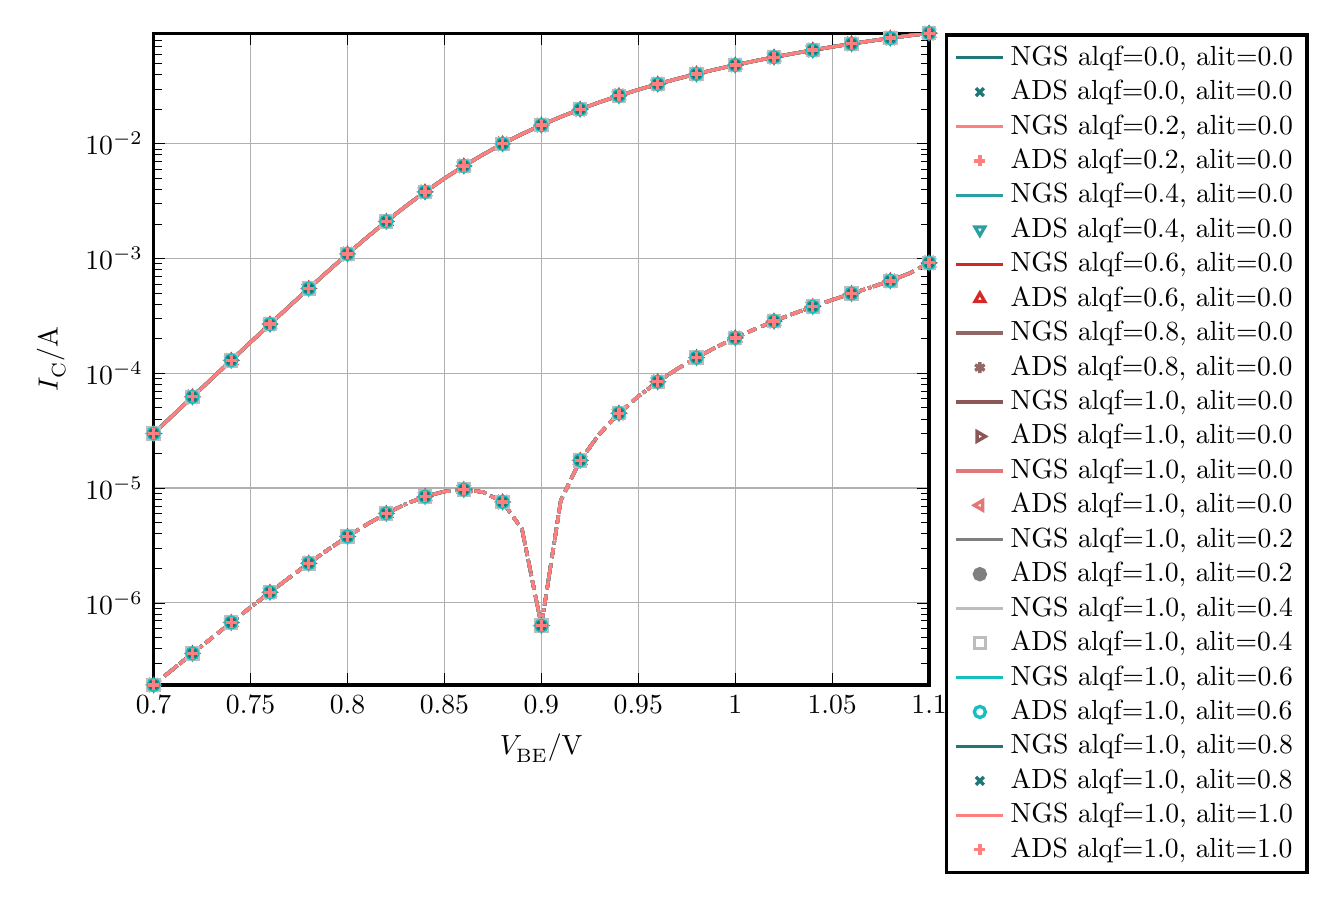
\begin{tikzpicture}[font=\normalsize]
\pgfplotsset{every axis/.append style={very thick}},
\definecolor{color0}{rgb}{0.12157, 0.46667, 0.46667}
\definecolor{color1}{rgb}{1.00000, 0.49804, 0.49804}
\definecolor{color2}{rgb}{0.17255, 0.62745, 0.62745}
\definecolor{color3}{rgb}{0.83922, 0.15294, 0.15294}
\definecolor{color4}{rgb}{0.58039, 0.40392, 0.40392}
\definecolor{color5}{rgb}{0.54902, 0.33725, 0.33725}
\definecolor{color6}{rgb}{0.89020, 0.46667, 0.46667}
\definecolor{color7}{rgb}{0.49804, 0.49804, 0.49804}
\definecolor{color8}{rgb}{0.73725, 0.74118, 0.74118}
\definecolor{color9}{rgb}{0.09020, 0.74510, 0.74510}

\begin{axis}[
width=4.5in,
xlabel={$V_{\mathrm{BE}}^{}/\si{\volt}$},
ylabel={$I_{\mathrm{C}}^{}/\si{\ampere}$},
ymode=log,
% xmin=0,
% xmax=0,
% restrict x to domain=0:1,
log basis x=10,
% ymin=0,
% ymax=0,
% restrict y to domain=0:1,
log basis y=10,
xmajorgrids,
enlargelimits=false,
scaled ticks=false,
ymajorgrids,
x tick style={color=black},
y tick style={color=black},
x grid style={white!69.01960784313725!black},
y grid style={white!69.01960784313725!black},
/tikz/mark repeat=2,
legend style={at={(1.02,1.00)}, anchor=north west,legend cell align=left, align=left},
]
\addplot [color=color0, solid,  mark phase=0, ]
  table[row sep=crcr, x expr=\thisrowno{0}*1.000000e+00, y expr=\thisrowno{1}*1.000000e+00]{
0.7 2.98396e-05\\
0.71 4.31177e-05\\
0.72 6.225e-05\\
0.73 8.97943e-05\\
0.74 0.000129401\\
0.75 0.000186243\\
0.76 0.000267564\\
0.77 0.000383354\\
0.78 0.000547084\\
0.79 0.000776382\\
0.8 0.00109339\\
0.81 0.00152451\\
0.82 0.00209913\\
0.83 0.00284735\\
0.84 0.00379703\\
0.85 0.00497087\\
0.86 0.00638447\\
0.87 0.00804567\\
0.88 0.0099552\\
0.89 0.012108\\
0.9 0.0144948\\
0.91 0.0171038\\
0.92 0.0199213\\
0.93 0.0229333\\
0.94 0.0261255\\
0.95 0.0294841\\
0.96 0.0329955\\
0.97 0.0366471\\
0.98 0.0404269\\
0.99 0.0443236\\
1 0.0483264\\
1.01 0.0524253\\
1.02 0.0566106\\
1.03 0.060873\\
1.04 0.0652035\\
1.05 0.0695925\\
1.06 0.0740296\\
1.07 0.0784992\\
1.08 0.08297\\
1.09 0.0873655\\
1.1 0.0915303\\
};
\addlegendentry{NGS alqf=0.0, alit=0.0}
\addplot [color=color0, only marks, mark=x, mark options={solid}, mark phase=0, ]
  table[row sep=crcr, x expr=\thisrowno{0}*1.000000e+00, y expr=\thisrowno{1}*1.000000e+00]{
0.7 2.98384e-05\\
0.71 4.31161e-05\\
0.72 6.22476e-05\\
0.73 8.97908e-05\\
0.74 0.000129396\\
0.75 0.000186236\\
0.76 0.000267554\\
0.77 0.000383339\\
0.78 0.000547063\\
0.79 0.000776351\\
0.8 0.00109335\\
0.81 0.00152446\\
0.82 0.00209905\\
0.83 0.00284725\\
0.84 0.0037969\\
0.85 0.00497072\\
0.86 0.00638428\\
0.87 0.00804546\\
0.88 0.00995495\\
0.89 0.0121077\\
0.9 0.0144945\\
0.91 0.0171034\\
0.92 0.019921\\
0.93 0.0229329\\
0.94 0.0261251\\
0.95 0.0294836\\
0.96 0.032995\\
0.97 0.0366466\\
0.98 0.0404264\\
0.99 0.0443231\\
1 0.0483259\\
1.01 0.0524248\\
1.02 0.0566101\\
1.03 0.0608725\\
1.04 0.0652029\\
1.05 0.069592\\
1.06 0.074029\\
1.07 0.0784986\\
1.08 0.0829694\\
1.09 0.0873649\\
1.1 0.0915297\\
};
\addlegendentry{ADS alqf=0.0, alit=0.0}
\addplot [color=color0, dashed,  mark phase=0, forget plot, ]
  table[row sep=crcr, x expr=\thisrowno{0}*1.000000e+00, y expr=\thisrowno{1}*1.000000e+00]{
0.7 1.92566e-07\\
0.71 2.64497e-07\\
0.72 3.62279e-07\\
0.73 4.94792e-07\\
0.74 6.737e-07\\
0.75 9.14018e-07\\
0.76 1.23452e-06\\
0.77 1.65766e-06\\
0.78 2.20837e-06\\
0.79 2.91096e-06\\
0.8 3.78297e-06\\
0.81 4.82508e-06\\
0.82 6.00723e-06\\
0.83 7.25302e-06\\
0.84 8.42655e-06\\
0.85 9.32676e-06\\
0.86 9.69201e-06\\
0.87 9.21432e-06\\
0.88 7.55919e-06\\
0.89 4.38615e-06\\
0.9 6.33686e-07\\
0.91 7.80474e-06\\
0.92 1.73992e-05\\
0.93 2.96533e-05\\
0.94 4.47678e-05\\
0.95 6.29099e-05\\
0.96 8.42176e-05\\
0.97 0.000108805\\
0.98 0.000136769\\
0.99 0.000168195\\
1 0.000203163\\
1.01 0.000241758\\
1.02 0.000284075\\
1.03 0.000330235\\
1.04 0.000380401\\
1.05 0.000434847\\
1.06 0.000494152\\
1.07 0.000559961\\
1.08 0.00063757\\
1.09 0.000743217\\
1.1 0.000914907\\
};
% \addlegendentry{}
\addplot [color=color0, dashdotted, mark=x, mark options={solid}, mark phase=0, forget plot, ]
  table[row sep=crcr, x expr=\thisrowno{0}*1.000000e+00, y expr=\thisrowno{1}*1.000000e+00]{
0.7 1.92559e-07\\
0.71 2.64488e-07\\
0.72 3.62265e-07\\
0.73 4.94774e-07\\
0.74 6.73673e-07\\
0.75 9.13982e-07\\
0.76 1.23448e-06\\
0.77 1.6576e-06\\
0.78 2.20828e-06\\
0.79 2.91085e-06\\
0.8 3.78283e-06\\
0.81 4.82491e-06\\
0.82 6.00703e-06\\
0.83 7.25279e-06\\
0.84 8.42632e-06\\
0.85 9.32655e-06\\
0.86 9.69185e-06\\
0.87 9.21425e-06\\
0.88 7.55926e-06\\
0.89 4.38638e-06\\
0.9 6.33234e-07\\
0.91 7.80403e-06\\
0.92 1.73982e-05\\
0.93 2.9652e-05\\
0.94 4.47661e-05\\
0.95 6.29078e-05\\
0.96 8.42152e-05\\
0.97 0.000108802\\
0.98 0.000136766\\
0.99 0.000168191\\
1 0.000203159\\
1.01 0.000241753\\
1.02 0.00028407\\
1.03 0.000330229\\
1.04 0.000380395\\
1.05 0.00043484\\
1.06 0.000494145\\
1.07 0.000559952\\
1.08 0.000637559\\
1.09 0.0007432\\
1.1 0.000914878\\
};
% \addlegendentry{}
\addplot [color=color1, solid,  mark phase=0, ]
  table[row sep=crcr, x expr=\thisrowno{0}*1.000000e+00, y expr=\thisrowno{1}*1.000000e+00]{
0.7 2.98396e-05\\
0.71 4.31177e-05\\
0.72 6.225e-05\\
0.73 8.97943e-05\\
0.74 0.000129401\\
0.75 0.000186243\\
0.76 0.000267564\\
0.77 0.000383354\\
0.78 0.000547084\\
0.79 0.000776382\\
0.8 0.00109339\\
0.81 0.00152451\\
0.82 0.00209913\\
0.83 0.00284735\\
0.84 0.00379703\\
0.85 0.00497087\\
0.86 0.00638447\\
0.87 0.00804567\\
0.88 0.0099552\\
0.89 0.012108\\
0.9 0.0144948\\
0.91 0.0171038\\
0.92 0.0199213\\
0.93 0.0229333\\
0.94 0.0261255\\
0.95 0.0294841\\
0.96 0.0329955\\
0.97 0.0366471\\
0.98 0.0404269\\
0.99 0.0443236\\
1 0.0483264\\
1.01 0.0524253\\
1.02 0.0566106\\
1.03 0.060873\\
1.04 0.0652035\\
1.05 0.0695925\\
1.06 0.0740296\\
1.07 0.0784992\\
1.08 0.08297\\
1.09 0.0873655\\
1.1 0.0915303\\
};
\addlegendentry{NGS alqf=0.2, alit=0.0}
\addplot [color=color1, only marks, mark=+, mark options={solid}, mark phase=0, ]
  table[row sep=crcr, x expr=\thisrowno{0}*1.000000e+00, y expr=\thisrowno{1}*1.000000e+00]{
0.7 2.98384e-05\\
0.71 4.31161e-05\\
0.72 6.22476e-05\\
0.73 8.97908e-05\\
0.74 0.000129396\\
0.75 0.000186236\\
0.76 0.000267554\\
0.77 0.000383339\\
0.78 0.000547063\\
0.79 0.000776351\\
0.8 0.00109335\\
0.81 0.00152446\\
0.82 0.00209905\\
0.83 0.00284725\\
0.84 0.0037969\\
0.85 0.00497072\\
0.86 0.00638428\\
0.87 0.00804546\\
0.88 0.00995495\\
0.89 0.0121077\\
0.9 0.0144945\\
0.91 0.0171034\\
0.92 0.019921\\
0.93 0.0229329\\
0.94 0.0261251\\
0.95 0.0294836\\
0.96 0.032995\\
0.97 0.0366466\\
0.98 0.0404264\\
0.99 0.0443231\\
1 0.0483259\\
1.01 0.0524248\\
1.02 0.0566101\\
1.03 0.0608725\\
1.04 0.0652029\\
1.05 0.069592\\
1.06 0.074029\\
1.07 0.0784986\\
1.08 0.0829694\\
1.09 0.0873649\\
1.1 0.0915297\\
};
\addlegendentry{ADS alqf=0.2, alit=0.0}
\addplot [color=color1, dashed,  mark phase=0, forget plot, ]
  table[row sep=crcr, x expr=\thisrowno{0}*1.000000e+00, y expr=\thisrowno{1}*1.000000e+00]{
0.7 1.92566e-07\\
0.71 2.64497e-07\\
0.72 3.62279e-07\\
0.73 4.94792e-07\\
0.74 6.737e-07\\
0.75 9.14018e-07\\
0.76 1.23452e-06\\
0.77 1.65766e-06\\
0.78 2.20837e-06\\
0.79 2.91096e-06\\
0.8 3.78297e-06\\
0.81 4.82508e-06\\
0.82 6.00723e-06\\
0.83 7.25302e-06\\
0.84 8.42655e-06\\
0.85 9.32676e-06\\
0.86 9.69201e-06\\
0.87 9.21432e-06\\
0.88 7.55919e-06\\
0.89 4.38615e-06\\
0.9 6.33687e-07\\
0.91 7.80474e-06\\
0.92 1.73992e-05\\
0.93 2.96533e-05\\
0.94 4.47678e-05\\
0.95 6.29099e-05\\
0.96 8.42176e-05\\
0.97 0.000108805\\
0.98 0.000136769\\
0.99 0.000168195\\
1 0.000203163\\
1.01 0.000241758\\
1.02 0.000284075\\
1.03 0.000330235\\
1.04 0.000380401\\
1.05 0.000434847\\
1.06 0.000494152\\
1.07 0.000559961\\
1.08 0.00063757\\
1.09 0.000743216\\
1.1 0.000914907\\
};
% \addlegendentry{}
\addplot [color=color1, dashdotted, mark=+, mark options={solid}, mark phase=0, forget plot, ]
  table[row sep=crcr, x expr=\thisrowno{0}*1.000000e+00, y expr=\thisrowno{1}*1.000000e+00]{
0.7 1.92559e-07\\
0.71 2.64488e-07\\
0.72 3.62265e-07\\
0.73 4.94774e-07\\
0.74 6.73673e-07\\
0.75 9.13982e-07\\
0.76 1.23448e-06\\
0.77 1.6576e-06\\
0.78 2.20828e-06\\
0.79 2.91085e-06\\
0.8 3.78283e-06\\
0.81 4.82491e-06\\
0.82 6.00703e-06\\
0.83 7.25279e-06\\
0.84 8.42632e-06\\
0.85 9.32655e-06\\
0.86 9.69185e-06\\
0.87 9.21425e-06\\
0.88 7.55926e-06\\
0.89 4.38638e-06\\
0.9 6.33234e-07\\
0.91 7.80403e-06\\
0.92 1.73982e-05\\
0.93 2.9652e-05\\
0.94 4.47661e-05\\
0.95 6.29078e-05\\
0.96 8.42152e-05\\
0.97 0.000108802\\
0.98 0.000136766\\
0.99 0.000168191\\
1 0.000203159\\
1.01 0.000241753\\
1.02 0.00028407\\
1.03 0.000330229\\
1.04 0.000380395\\
1.05 0.00043484\\
1.06 0.000494145\\
1.07 0.000559952\\
1.08 0.000637559\\
1.09 0.0007432\\
1.1 0.000914878\\
};
% \addlegendentry{}
\addplot [color=color2, solid,  mark phase=0, ]
  table[row sep=crcr, x expr=\thisrowno{0}*1.000000e+00, y expr=\thisrowno{1}*1.000000e+00]{
0.7 2.98396e-05\\
0.71 4.31177e-05\\
0.72 6.225e-05\\
0.73 8.97943e-05\\
0.74 0.000129401\\
0.75 0.000186243\\
0.76 0.000267564\\
0.77 0.000383354\\
0.78 0.000547084\\
0.79 0.000776382\\
0.8 0.00109339\\
0.81 0.00152451\\
0.82 0.00209913\\
0.83 0.00284735\\
0.84 0.00379703\\
0.85 0.00497087\\
0.86 0.00638447\\
0.87 0.00804567\\
0.88 0.0099552\\
0.89 0.012108\\
0.9 0.0144948\\
0.91 0.0171038\\
0.92 0.0199213\\
0.93 0.0229333\\
0.94 0.0261255\\
0.95 0.0294841\\
0.96 0.0329955\\
0.97 0.0366471\\
0.98 0.0404269\\
0.99 0.0443236\\
1 0.0483264\\
1.01 0.0524253\\
1.02 0.0566106\\
1.03 0.060873\\
1.04 0.0652035\\
1.05 0.0695925\\
1.06 0.0740296\\
1.07 0.0784992\\
1.08 0.08297\\
1.09 0.0873655\\
1.1 0.0915303\\
};
\addlegendentry{NGS alqf=0.4, alit=0.0}
\addplot [color=color2, only marks, mark=triangle, mark options={solid, rotate=180}, mark phase=0, ]
  table[row sep=crcr, x expr=\thisrowno{0}*1.000000e+00, y expr=\thisrowno{1}*1.000000e+00]{
0.7 2.98384e-05\\
0.71 4.31161e-05\\
0.72 6.22476e-05\\
0.73 8.97908e-05\\
0.74 0.000129396\\
0.75 0.000186236\\
0.76 0.000267554\\
0.77 0.000383339\\
0.78 0.000547063\\
0.79 0.000776351\\
0.8 0.00109335\\
0.81 0.00152446\\
0.82 0.00209905\\
0.83 0.00284725\\
0.84 0.0037969\\
0.85 0.00497072\\
0.86 0.00638428\\
0.87 0.00804546\\
0.88 0.00995495\\
0.89 0.0121077\\
0.9 0.0144945\\
0.91 0.0171034\\
0.92 0.019921\\
0.93 0.0229329\\
0.94 0.0261251\\
0.95 0.0294836\\
0.96 0.032995\\
0.97 0.0366466\\
0.98 0.0404264\\
0.99 0.0443231\\
1 0.0483259\\
1.01 0.0524248\\
1.02 0.0566101\\
1.03 0.0608725\\
1.04 0.0652029\\
1.05 0.069592\\
1.06 0.074029\\
1.07 0.0784986\\
1.08 0.0829694\\
1.09 0.0873649\\
1.1 0.0915297\\
};
\addlegendentry{ADS alqf=0.4, alit=0.0}
\addplot [color=color2, dashed,  mark phase=0, forget plot, ]
  table[row sep=crcr, x expr=\thisrowno{0}*1.000000e+00, y expr=\thisrowno{1}*1.000000e+00]{
0.7 1.92566e-07\\
0.71 2.64497e-07\\
0.72 3.62279e-07\\
0.73 4.94792e-07\\
0.74 6.737e-07\\
0.75 9.14018e-07\\
0.76 1.23452e-06\\
0.77 1.65766e-06\\
0.78 2.20837e-06\\
0.79 2.91096e-06\\
0.8 3.78297e-06\\
0.81 4.82508e-06\\
0.82 6.00723e-06\\
0.83 7.25302e-06\\
0.84 8.42655e-06\\
0.85 9.32676e-06\\
0.86 9.69201e-06\\
0.87 9.21432e-06\\
0.88 7.55919e-06\\
0.89 4.38615e-06\\
0.9 6.33687e-07\\
0.91 7.80474e-06\\
0.92 1.73992e-05\\
0.93 2.96533e-05\\
0.94 4.47678e-05\\
0.95 6.29099e-05\\
0.96 8.42176e-05\\
0.97 0.000108805\\
0.98 0.000136769\\
0.99 0.000168195\\
1 0.000203163\\
1.01 0.000241758\\
1.02 0.000284075\\
1.03 0.000330235\\
1.04 0.000380401\\
1.05 0.000434847\\
1.06 0.000494152\\
1.07 0.000559961\\
1.08 0.00063757\\
1.09 0.000743216\\
1.1 0.000914907\\
};
% \addlegendentry{}
\addplot [color=color2, dashdotted, mark=triangle, mark options={solid, rotate=180}, mark phase=0, forget plot, ]
  table[row sep=crcr, x expr=\thisrowno{0}*1.000000e+00, y expr=\thisrowno{1}*1.000000e+00]{
0.7 1.92559e-07\\
0.71 2.64488e-07\\
0.72 3.62265e-07\\
0.73 4.94774e-07\\
0.74 6.73673e-07\\
0.75 9.13982e-07\\
0.76 1.23448e-06\\
0.77 1.6576e-06\\
0.78 2.20828e-06\\
0.79 2.91085e-06\\
0.8 3.78283e-06\\
0.81 4.82491e-06\\
0.82 6.00703e-06\\
0.83 7.25279e-06\\
0.84 8.42632e-06\\
0.85 9.32655e-06\\
0.86 9.69185e-06\\
0.87 9.21425e-06\\
0.88 7.55926e-06\\
0.89 4.38638e-06\\
0.9 6.33234e-07\\
0.91 7.80403e-06\\
0.92 1.73982e-05\\
0.93 2.9652e-05\\
0.94 4.47661e-05\\
0.95 6.29078e-05\\
0.96 8.42152e-05\\
0.97 0.000108802\\
0.98 0.000136766\\
0.99 0.000168191\\
1 0.000203159\\
1.01 0.000241753\\
1.02 0.00028407\\
1.03 0.000330229\\
1.04 0.000380395\\
1.05 0.00043484\\
1.06 0.000494145\\
1.07 0.000559952\\
1.08 0.000637559\\
1.09 0.0007432\\
1.1 0.000914878\\
};
% \addlegendentry{}
\addplot [color=color3, solid,  mark phase=0, ]
  table[row sep=crcr, x expr=\thisrowno{0}*1.000000e+00, y expr=\thisrowno{1}*1.000000e+00]{
0.7 2.98396e-05\\
0.71 4.31177e-05\\
0.72 6.225e-05\\
0.73 8.97943e-05\\
0.74 0.000129401\\
0.75 0.000186243\\
0.76 0.000267564\\
0.77 0.000383354\\
0.78 0.000547084\\
0.79 0.000776382\\
0.8 0.00109339\\
0.81 0.00152451\\
0.82 0.00209913\\
0.83 0.00284735\\
0.84 0.00379703\\
0.85 0.00497087\\
0.86 0.00638447\\
0.87 0.00804567\\
0.88 0.0099552\\
0.89 0.012108\\
0.9 0.0144948\\
0.91 0.0171038\\
0.92 0.0199213\\
0.93 0.0229333\\
0.94 0.0261255\\
0.95 0.0294841\\
0.96 0.0329955\\
0.97 0.0366471\\
0.98 0.0404269\\
0.99 0.0443236\\
1 0.0483264\\
1.01 0.0524253\\
1.02 0.0566106\\
1.03 0.060873\\
1.04 0.0652035\\
1.05 0.0695925\\
1.06 0.0740296\\
1.07 0.0784992\\
1.08 0.08297\\
1.09 0.0873655\\
1.1 0.0915303\\
};
\addlegendentry{NGS alqf=0.6, alit=0.0}
\addplot [color=color3, only marks, mark=triangle, mark options={solid, rotate=0}, mark phase=0, ]
  table[row sep=crcr, x expr=\thisrowno{0}*1.000000e+00, y expr=\thisrowno{1}*1.000000e+00]{
0.7 2.98384e-05\\
0.71 4.31161e-05\\
0.72 6.22476e-05\\
0.73 8.97908e-05\\
0.74 0.000129396\\
0.75 0.000186236\\
0.76 0.000267554\\
0.77 0.000383339\\
0.78 0.000547063\\
0.79 0.000776351\\
0.8 0.00109335\\
0.81 0.00152446\\
0.82 0.00209905\\
0.83 0.00284725\\
0.84 0.0037969\\
0.85 0.00497072\\
0.86 0.00638428\\
0.87 0.00804546\\
0.88 0.00995495\\
0.89 0.0121077\\
0.9 0.0144945\\
0.91 0.0171034\\
0.92 0.019921\\
0.93 0.0229329\\
0.94 0.0261251\\
0.95 0.0294836\\
0.96 0.032995\\
0.97 0.0366466\\
0.98 0.0404264\\
0.99 0.0443231\\
1 0.0483259\\
1.01 0.0524248\\
1.02 0.0566101\\
1.03 0.0608725\\
1.04 0.0652029\\
1.05 0.069592\\
1.06 0.074029\\
1.07 0.0784986\\
1.08 0.0829694\\
1.09 0.0873649\\
1.1 0.0915297\\
};
\addlegendentry{ADS alqf=0.6, alit=0.0}
\addplot [color=color3, dashed,  mark phase=0, forget plot, ]
  table[row sep=crcr, x expr=\thisrowno{0}*1.000000e+00, y expr=\thisrowno{1}*1.000000e+00]{
0.7 1.92566e-07\\
0.71 2.64497e-07\\
0.72 3.62279e-07\\
0.73 4.94792e-07\\
0.74 6.737e-07\\
0.75 9.14018e-07\\
0.76 1.23452e-06\\
0.77 1.65766e-06\\
0.78 2.20837e-06\\
0.79 2.91096e-06\\
0.8 3.78297e-06\\
0.81 4.82508e-06\\
0.82 6.00723e-06\\
0.83 7.25302e-06\\
0.84 8.42655e-06\\
0.85 9.32676e-06\\
0.86 9.69201e-06\\
0.87 9.21432e-06\\
0.88 7.55919e-06\\
0.89 4.38615e-06\\
0.9 6.33687e-07\\
0.91 7.80474e-06\\
0.92 1.73992e-05\\
0.93 2.96533e-05\\
0.94 4.47678e-05\\
0.95 6.29099e-05\\
0.96 8.42176e-05\\
0.97 0.000108805\\
0.98 0.000136769\\
0.99 0.000168195\\
1 0.000203163\\
1.01 0.000241758\\
1.02 0.000284075\\
1.03 0.000330235\\
1.04 0.000380401\\
1.05 0.000434847\\
1.06 0.000494152\\
1.07 0.000559961\\
1.08 0.00063757\\
1.09 0.000743216\\
1.1 0.000914907\\
};
% \addlegendentry{}
\addplot [color=color3, dashdotted, mark=triangle, mark options={solid, rotate=0}, mark phase=0, forget plot, ]
  table[row sep=crcr, x expr=\thisrowno{0}*1.000000e+00, y expr=\thisrowno{1}*1.000000e+00]{
0.7 1.92559e-07\\
0.71 2.64488e-07\\
0.72 3.62265e-07\\
0.73 4.94774e-07\\
0.74 6.73673e-07\\
0.75 9.13982e-07\\
0.76 1.23448e-06\\
0.77 1.6576e-06\\
0.78 2.20828e-06\\
0.79 2.91085e-06\\
0.8 3.78283e-06\\
0.81 4.82491e-06\\
0.82 6.00703e-06\\
0.83 7.25279e-06\\
0.84 8.42632e-06\\
0.85 9.32655e-06\\
0.86 9.69185e-06\\
0.87 9.21425e-06\\
0.88 7.55926e-06\\
0.89 4.38638e-06\\
0.9 6.33234e-07\\
0.91 7.80403e-06\\
0.92 1.73982e-05\\
0.93 2.9652e-05\\
0.94 4.47661e-05\\
0.95 6.29078e-05\\
0.96 8.42152e-05\\
0.97 0.000108802\\
0.98 0.000136766\\
0.99 0.000168191\\
1 0.000203159\\
1.01 0.000241753\\
1.02 0.00028407\\
1.03 0.000330229\\
1.04 0.000380395\\
1.05 0.00043484\\
1.06 0.000494145\\
1.07 0.000559952\\
1.08 0.000637559\\
1.09 0.0007432\\
1.1 0.000914878\\
};
% \addlegendentry{}
\addplot [color=color4, solid,  mark phase=0, ]
  table[row sep=crcr, x expr=\thisrowno{0}*1.000000e+00, y expr=\thisrowno{1}*1.000000e+00]{
0.7 2.98396e-05\\
0.71 4.31177e-05\\
0.72 6.225e-05\\
0.73 8.97943e-05\\
0.74 0.000129401\\
0.75 0.000186243\\
0.76 0.000267564\\
0.77 0.000383354\\
0.78 0.000547084\\
0.79 0.000776382\\
0.8 0.00109339\\
0.81 0.00152451\\
0.82 0.00209913\\
0.83 0.00284735\\
0.84 0.00379703\\
0.85 0.00497087\\
0.86 0.00638447\\
0.87 0.00804567\\
0.88 0.0099552\\
0.89 0.012108\\
0.9 0.0144948\\
0.91 0.0171038\\
0.92 0.0199213\\
0.93 0.0229333\\
0.94 0.0261255\\
0.95 0.0294841\\
0.96 0.0329955\\
0.97 0.0366471\\
0.98 0.0404269\\
0.99 0.0443236\\
1 0.0483264\\
1.01 0.0524253\\
1.02 0.0566106\\
1.03 0.060873\\
1.04 0.0652035\\
1.05 0.0695925\\
1.06 0.0740296\\
1.07 0.0784992\\
1.08 0.08297\\
1.09 0.0873655\\
1.1 0.0915303\\
};
\addlegendentry{NGS alqf=0.8, alit=0.0}
\addplot [color=color4, only marks, mark=asterisk, mark options={solid}, mark phase=0, ]
  table[row sep=crcr, x expr=\thisrowno{0}*1.000000e+00, y expr=\thisrowno{1}*1.000000e+00]{
0.7 2.98384e-05\\
0.71 4.31161e-05\\
0.72 6.22476e-05\\
0.73 8.97908e-05\\
0.74 0.000129396\\
0.75 0.000186236\\
0.76 0.000267554\\
0.77 0.000383339\\
0.78 0.000547063\\
0.79 0.000776351\\
0.8 0.00109335\\
0.81 0.00152446\\
0.82 0.00209905\\
0.83 0.00284725\\
0.84 0.0037969\\
0.85 0.00497072\\
0.86 0.00638428\\
0.87 0.00804546\\
0.88 0.00995495\\
0.89 0.0121077\\
0.9 0.0144945\\
0.91 0.0171034\\
0.92 0.019921\\
0.93 0.0229329\\
0.94 0.0261251\\
0.95 0.0294836\\
0.96 0.032995\\
0.97 0.0366466\\
0.98 0.0404264\\
0.99 0.0443231\\
1 0.0483259\\
1.01 0.0524248\\
1.02 0.0566101\\
1.03 0.0608725\\
1.04 0.0652029\\
1.05 0.069592\\
1.06 0.074029\\
1.07 0.0784986\\
1.08 0.0829694\\
1.09 0.0873649\\
1.1 0.0915297\\
};
\addlegendentry{ADS alqf=0.8, alit=0.0}
\addplot [color=color4, dashed,  mark phase=0, forget plot, ]
  table[row sep=crcr, x expr=\thisrowno{0}*1.000000e+00, y expr=\thisrowno{1}*1.000000e+00]{
0.7 1.92566e-07\\
0.71 2.64497e-07\\
0.72 3.62279e-07\\
0.73 4.94792e-07\\
0.74 6.737e-07\\
0.75 9.14018e-07\\
0.76 1.23452e-06\\
0.77 1.65766e-06\\
0.78 2.20837e-06\\
0.79 2.91096e-06\\
0.8 3.78297e-06\\
0.81 4.82508e-06\\
0.82 6.00723e-06\\
0.83 7.25302e-06\\
0.84 8.42655e-06\\
0.85 9.32676e-06\\
0.86 9.69201e-06\\
0.87 9.21432e-06\\
0.88 7.55919e-06\\
0.89 4.38615e-06\\
0.9 6.33687e-07\\
0.91 7.80474e-06\\
0.92 1.73992e-05\\
0.93 2.96533e-05\\
0.94 4.47678e-05\\
0.95 6.29099e-05\\
0.96 8.42176e-05\\
0.97 0.000108805\\
0.98 0.000136769\\
0.99 0.000168195\\
1 0.000203163\\
1.01 0.000241758\\
1.02 0.000284075\\
1.03 0.000330235\\
1.04 0.000380401\\
1.05 0.000434847\\
1.06 0.000494152\\
1.07 0.000559961\\
1.08 0.00063757\\
1.09 0.000743216\\
1.1 0.000914907\\
};
% \addlegendentry{}
\addplot [color=color4, dashdotted, mark=asterisk, mark options={solid}, mark phase=0, forget plot, ]
  table[row sep=crcr, x expr=\thisrowno{0}*1.000000e+00, y expr=\thisrowno{1}*1.000000e+00]{
0.7 1.92559e-07\\
0.71 2.64488e-07\\
0.72 3.62265e-07\\
0.73 4.94774e-07\\
0.74 6.73673e-07\\
0.75 9.13982e-07\\
0.76 1.23448e-06\\
0.77 1.6576e-06\\
0.78 2.20828e-06\\
0.79 2.91085e-06\\
0.8 3.78283e-06\\
0.81 4.82491e-06\\
0.82 6.00703e-06\\
0.83 7.25279e-06\\
0.84 8.42632e-06\\
0.85 9.32655e-06\\
0.86 9.69185e-06\\
0.87 9.21425e-06\\
0.88 7.55926e-06\\
0.89 4.38638e-06\\
0.9 6.33234e-07\\
0.91 7.80403e-06\\
0.92 1.73982e-05\\
0.93 2.9652e-05\\
0.94 4.47661e-05\\
0.95 6.29078e-05\\
0.96 8.42152e-05\\
0.97 0.000108802\\
0.98 0.000136766\\
0.99 0.000168191\\
1 0.000203159\\
1.01 0.000241753\\
1.02 0.00028407\\
1.03 0.000330229\\
1.04 0.000380395\\
1.05 0.00043484\\
1.06 0.000494145\\
1.07 0.000559952\\
1.08 0.000637559\\
1.09 0.0007432\\
1.1 0.000914878\\
};
% \addlegendentry{}
\addplot [color=color5, solid,  mark phase=0, ]
  table[row sep=crcr, x expr=\thisrowno{0}*1.000000e+00, y expr=\thisrowno{1}*1.000000e+00]{
0.7 2.98396e-05\\
0.71 4.31177e-05\\
0.72 6.225e-05\\
0.73 8.97943e-05\\
0.74 0.000129401\\
0.75 0.000186243\\
0.76 0.000267564\\
0.77 0.000383354\\
0.78 0.000547084\\
0.79 0.000776382\\
0.8 0.00109339\\
0.81 0.00152451\\
0.82 0.00209913\\
0.83 0.00284735\\
0.84 0.00379703\\
0.85 0.00497087\\
0.86 0.00638447\\
0.87 0.00804567\\
0.88 0.0099552\\
0.89 0.012108\\
0.9 0.0144948\\
0.91 0.0171038\\
0.92 0.0199213\\
0.93 0.0229333\\
0.94 0.0261255\\
0.95 0.0294841\\
0.96 0.0329955\\
0.97 0.0366471\\
0.98 0.0404269\\
0.99 0.0443236\\
1 0.0483264\\
1.01 0.0524253\\
1.02 0.0566106\\
1.03 0.060873\\
1.04 0.0652035\\
1.05 0.0695925\\
1.06 0.0740296\\
1.07 0.0784992\\
1.08 0.08297\\
1.09 0.0873655\\
1.1 0.0915303\\
};
\addlegendentry{NGS alqf=1.0, alit=0.0}
\addplot [color=color5, only marks, mark=triangle, mark options={solid, rotate=270}, mark phase=0, ]
  table[row sep=crcr, x expr=\thisrowno{0}*1.000000e+00, y expr=\thisrowno{1}*1.000000e+00]{
0.7 2.98384e-05\\
0.71 4.31161e-05\\
0.72 6.22476e-05\\
0.73 8.97908e-05\\
0.74 0.000129396\\
0.75 0.000186236\\
0.76 0.000267554\\
0.77 0.000383339\\
0.78 0.000547063\\
0.79 0.000776351\\
0.8 0.00109335\\
0.81 0.00152446\\
0.82 0.00209905\\
0.83 0.00284725\\
0.84 0.0037969\\
0.85 0.00497072\\
0.86 0.00638428\\
0.87 0.00804546\\
0.88 0.00995495\\
0.89 0.0121077\\
0.9 0.0144945\\
0.91 0.0171034\\
0.92 0.019921\\
0.93 0.0229329\\
0.94 0.0261251\\
0.95 0.0294836\\
0.96 0.032995\\
0.97 0.0366466\\
0.98 0.0404264\\
0.99 0.0443231\\
1 0.0483259\\
1.01 0.0524248\\
1.02 0.0566101\\
1.03 0.0608725\\
1.04 0.0652029\\
1.05 0.069592\\
1.06 0.074029\\
1.07 0.0784986\\
1.08 0.0829694\\
1.09 0.0873649\\
1.1 0.0915297\\
};
\addlegendentry{ADS alqf=1.0, alit=0.0}
\addplot [color=color5, dashed,  mark phase=0, forget plot, ]
  table[row sep=crcr, x expr=\thisrowno{0}*1.000000e+00, y expr=\thisrowno{1}*1.000000e+00]{
0.7 1.92566e-07\\
0.71 2.64497e-07\\
0.72 3.62279e-07\\
0.73 4.94792e-07\\
0.74 6.737e-07\\
0.75 9.14018e-07\\
0.76 1.23452e-06\\
0.77 1.65766e-06\\
0.78 2.20837e-06\\
0.79 2.91096e-06\\
0.8 3.78297e-06\\
0.81 4.82508e-06\\
0.82 6.00723e-06\\
0.83 7.25302e-06\\
0.84 8.42655e-06\\
0.85 9.32676e-06\\
0.86 9.69201e-06\\
0.87 9.21432e-06\\
0.88 7.55919e-06\\
0.89 4.38615e-06\\
0.9 6.33687e-07\\
0.91 7.80474e-06\\
0.92 1.73992e-05\\
0.93 2.96533e-05\\
0.94 4.47678e-05\\
0.95 6.29099e-05\\
0.96 8.42176e-05\\
0.97 0.000108805\\
0.98 0.000136769\\
0.99 0.000168195\\
1 0.000203163\\
1.01 0.000241758\\
1.02 0.000284075\\
1.03 0.000330235\\
1.04 0.000380401\\
1.05 0.000434847\\
1.06 0.000494152\\
1.07 0.000559961\\
1.08 0.00063757\\
1.09 0.000743216\\
1.1 0.000914907\\
};
% \addlegendentry{}
\addplot [color=color5, dashdotted, mark=triangle, mark options={solid, rotate=270}, mark phase=0, forget plot, ]
  table[row sep=crcr, x expr=\thisrowno{0}*1.000000e+00, y expr=\thisrowno{1}*1.000000e+00]{
0.7 1.92559e-07\\
0.71 2.64488e-07\\
0.72 3.62265e-07\\
0.73 4.94774e-07\\
0.74 6.73673e-07\\
0.75 9.13982e-07\\
0.76 1.23448e-06\\
0.77 1.6576e-06\\
0.78 2.20828e-06\\
0.79 2.91085e-06\\
0.8 3.78283e-06\\
0.81 4.82491e-06\\
0.82 6.00703e-06\\
0.83 7.25279e-06\\
0.84 8.42632e-06\\
0.85 9.32655e-06\\
0.86 9.69185e-06\\
0.87 9.21425e-06\\
0.88 7.55926e-06\\
0.89 4.38638e-06\\
0.9 6.33234e-07\\
0.91 7.80403e-06\\
0.92 1.73982e-05\\
0.93 2.9652e-05\\
0.94 4.47661e-05\\
0.95 6.29078e-05\\
0.96 8.42152e-05\\
0.97 0.000108802\\
0.98 0.000136766\\
0.99 0.000168191\\
1 0.000203159\\
1.01 0.000241753\\
1.02 0.00028407\\
1.03 0.000330229\\
1.04 0.000380395\\
1.05 0.00043484\\
1.06 0.000494145\\
1.07 0.000559952\\
1.08 0.000637559\\
1.09 0.0007432\\
1.1 0.000914878\\
};
% \addlegendentry{}
\addplot [color=color6, solid,  mark phase=0, ]
  table[row sep=crcr, x expr=\thisrowno{0}*1.000000e+00, y expr=\thisrowno{1}*1.000000e+00]{
0.7 2.98396e-05\\
0.71 4.31177e-05\\
0.72 6.225e-05\\
0.73 8.97943e-05\\
0.74 0.000129401\\
0.75 0.000186243\\
0.76 0.000267564\\
0.77 0.000383354\\
0.78 0.000547084\\
0.79 0.000776382\\
0.8 0.00109339\\
0.81 0.00152451\\
0.82 0.00209913\\
0.83 0.00284735\\
0.84 0.00379703\\
0.85 0.00497087\\
0.86 0.00638447\\
0.87 0.00804567\\
0.88 0.0099552\\
0.89 0.012108\\
0.9 0.0144948\\
0.91 0.0171038\\
0.92 0.0199213\\
0.93 0.0229333\\
0.94 0.0261255\\
0.95 0.0294841\\
0.96 0.0329955\\
0.97 0.0366471\\
0.98 0.0404269\\
0.99 0.0443236\\
1 0.0483264\\
1.01 0.0524253\\
1.02 0.0566106\\
1.03 0.060873\\
1.04 0.0652035\\
1.05 0.0695925\\
1.06 0.0740296\\
1.07 0.0784992\\
1.08 0.08297\\
1.09 0.0873655\\
1.1 0.0915303\\
};
\addlegendentry{NGS alqf=1.0, alit=0.0}
\addplot [color=color6, only marks, mark=triangle, mark options={solid, rotate=90}, mark phase=0, ]
  table[row sep=crcr, x expr=\thisrowno{0}*1.000000e+00, y expr=\thisrowno{1}*1.000000e+00]{
0.7 2.98384e-05\\
0.71 4.31161e-05\\
0.72 6.22476e-05\\
0.73 8.97908e-05\\
0.74 0.000129396\\
0.75 0.000186236\\
0.76 0.000267554\\
0.77 0.000383339\\
0.78 0.000547063\\
0.79 0.000776351\\
0.8 0.00109335\\
0.81 0.00152446\\
0.82 0.00209905\\
0.83 0.00284725\\
0.84 0.0037969\\
0.85 0.00497072\\
0.86 0.00638428\\
0.87 0.00804546\\
0.88 0.00995495\\
0.89 0.0121077\\
0.9 0.0144945\\
0.91 0.0171034\\
0.92 0.019921\\
0.93 0.0229329\\
0.94 0.0261251\\
0.95 0.0294836\\
0.96 0.032995\\
0.97 0.0366466\\
0.98 0.0404264\\
0.99 0.0443231\\
1 0.0483259\\
1.01 0.0524248\\
1.02 0.0566101\\
1.03 0.0608725\\
1.04 0.0652029\\
1.05 0.069592\\
1.06 0.074029\\
1.07 0.0784986\\
1.08 0.0829694\\
1.09 0.0873649\\
1.1 0.0915297\\
};
\addlegendentry{ADS alqf=1.0, alit=0.0}
\addplot [color=color6, dashed,  mark phase=0, forget plot, ]
  table[row sep=crcr, x expr=\thisrowno{0}*1.000000e+00, y expr=\thisrowno{1}*1.000000e+00]{
0.7 1.92566e-07\\
0.71 2.64497e-07\\
0.72 3.62279e-07\\
0.73 4.94792e-07\\
0.74 6.737e-07\\
0.75 9.14018e-07\\
0.76 1.23452e-06\\
0.77 1.65766e-06\\
0.78 2.20837e-06\\
0.79 2.91096e-06\\
0.8 3.78297e-06\\
0.81 4.82508e-06\\
0.82 6.00723e-06\\
0.83 7.25302e-06\\
0.84 8.42655e-06\\
0.85 9.32676e-06\\
0.86 9.69201e-06\\
0.87 9.21432e-06\\
0.88 7.55919e-06\\
0.89 4.38615e-06\\
0.9 6.33687e-07\\
0.91 7.80474e-06\\
0.92 1.73992e-05\\
0.93 2.96533e-05\\
0.94 4.47678e-05\\
0.95 6.29099e-05\\
0.96 8.42176e-05\\
0.97 0.000108805\\
0.98 0.000136769\\
0.99 0.000168195\\
1 0.000203163\\
1.01 0.000241758\\
1.02 0.000284075\\
1.03 0.000330235\\
1.04 0.000380401\\
1.05 0.000434847\\
1.06 0.000494152\\
1.07 0.000559961\\
1.08 0.00063757\\
1.09 0.000743216\\
1.1 0.000914907\\
};
% \addlegendentry{}
\addplot [color=color6, dashdotted, mark=triangle, mark options={solid, rotate=90}, mark phase=0, forget plot, ]
  table[row sep=crcr, x expr=\thisrowno{0}*1.000000e+00, y expr=\thisrowno{1}*1.000000e+00]{
0.7 1.92559e-07\\
0.71 2.64488e-07\\
0.72 3.62265e-07\\
0.73 4.94774e-07\\
0.74 6.73673e-07\\
0.75 9.13982e-07\\
0.76 1.23448e-06\\
0.77 1.6576e-06\\
0.78 2.20828e-06\\
0.79 2.91085e-06\\
0.8 3.78283e-06\\
0.81 4.82491e-06\\
0.82 6.00703e-06\\
0.83 7.25279e-06\\
0.84 8.42632e-06\\
0.85 9.32655e-06\\
0.86 9.69185e-06\\
0.87 9.21425e-06\\
0.88 7.55926e-06\\
0.89 4.38638e-06\\
0.9 6.33234e-07\\
0.91 7.80403e-06\\
0.92 1.73982e-05\\
0.93 2.9652e-05\\
0.94 4.47661e-05\\
0.95 6.29078e-05\\
0.96 8.42152e-05\\
0.97 0.000108802\\
0.98 0.000136766\\
0.99 0.000168191\\
1 0.000203159\\
1.01 0.000241753\\
1.02 0.00028407\\
1.03 0.000330229\\
1.04 0.000380395\\
1.05 0.00043484\\
1.06 0.000494145\\
1.07 0.000559952\\
1.08 0.000637559\\
1.09 0.0007432\\
1.1 0.000914878\\
};
% \addlegendentry{}
\addplot [color=color7, solid,  mark phase=0, ]
  table[row sep=crcr, x expr=\thisrowno{0}*1.000000e+00, y expr=\thisrowno{1}*1.000000e+00]{
0.7 2.98396e-05\\
0.71 4.31177e-05\\
0.72 6.225e-05\\
0.73 8.97943e-05\\
0.74 0.000129401\\
0.75 0.000186243\\
0.76 0.000267564\\
0.77 0.000383354\\
0.78 0.000547084\\
0.79 0.000776382\\
0.8 0.00109339\\
0.81 0.00152451\\
0.82 0.00209913\\
0.83 0.00284735\\
0.84 0.00379703\\
0.85 0.00497087\\
0.86 0.00638447\\
0.87 0.00804567\\
0.88 0.0099552\\
0.89 0.012108\\
0.9 0.0144948\\
0.91 0.0171038\\
0.92 0.0199213\\
0.93 0.0229333\\
0.94 0.0261255\\
0.95 0.0294841\\
0.96 0.0329955\\
0.97 0.0366471\\
0.98 0.0404269\\
0.99 0.0443236\\
1 0.0483264\\
1.01 0.0524253\\
1.02 0.0566106\\
1.03 0.060873\\
1.04 0.0652035\\
1.05 0.0695925\\
1.06 0.0740296\\
1.07 0.0784992\\
1.08 0.08297\\
1.09 0.0873655\\
1.1 0.0915303\\
};
\addlegendentry{NGS alqf=1.0, alit=0.2}
\addplot [color=color7, only marks, mark=*, mark options={solid, fill}, mark phase=0, ]
  table[row sep=crcr, x expr=\thisrowno{0}*1.000000e+00, y expr=\thisrowno{1}*1.000000e+00]{
0.7 2.98384e-05\\
0.71 4.31161e-05\\
0.72 6.22476e-05\\
0.73 8.97908e-05\\
0.74 0.000129396\\
0.75 0.000186236\\
0.76 0.000267554\\
0.77 0.000383339\\
0.78 0.000547063\\
0.79 0.000776351\\
0.8 0.00109335\\
0.81 0.00152446\\
0.82 0.00209905\\
0.83 0.00284725\\
0.84 0.0037969\\
0.85 0.00497072\\
0.86 0.00638428\\
0.87 0.00804546\\
0.88 0.00995495\\
0.89 0.0121077\\
0.9 0.0144945\\
0.91 0.0171034\\
0.92 0.019921\\
0.93 0.0229329\\
0.94 0.0261251\\
0.95 0.0294836\\
0.96 0.032995\\
0.97 0.0366466\\
0.98 0.0404264\\
0.99 0.0443231\\
1 0.0483259\\
1.01 0.0524248\\
1.02 0.0566101\\
1.03 0.0608725\\
1.04 0.0652029\\
1.05 0.069592\\
1.06 0.074029\\
1.07 0.0784986\\
1.08 0.0829694\\
1.09 0.0873649\\
1.1 0.0915297\\
};
\addlegendentry{ADS alqf=1.0, alit=0.2}
\addplot [color=color7, dashed,  mark phase=0, forget plot, ]
  table[row sep=crcr, x expr=\thisrowno{0}*1.000000e+00, y expr=\thisrowno{1}*1.000000e+00]{
0.7 1.92566e-07\\
0.71 2.64497e-07\\
0.72 3.62279e-07\\
0.73 4.94792e-07\\
0.74 6.737e-07\\
0.75 9.14018e-07\\
0.76 1.23452e-06\\
0.77 1.65766e-06\\
0.78 2.20837e-06\\
0.79 2.91096e-06\\
0.8 3.78297e-06\\
0.81 4.82508e-06\\
0.82 6.00723e-06\\
0.83 7.25302e-06\\
0.84 8.42655e-06\\
0.85 9.32676e-06\\
0.86 9.69201e-06\\
0.87 9.21432e-06\\
0.88 7.55919e-06\\
0.89 4.38615e-06\\
0.9 6.33687e-07\\
0.91 7.80474e-06\\
0.92 1.73992e-05\\
0.93 2.96533e-05\\
0.94 4.47678e-05\\
0.95 6.29099e-05\\
0.96 8.42176e-05\\
0.97 0.000108805\\
0.98 0.000136769\\
0.99 0.000168195\\
1 0.000203163\\
1.01 0.000241758\\
1.02 0.000284075\\
1.03 0.000330235\\
1.04 0.000380401\\
1.05 0.000434847\\
1.06 0.000494152\\
1.07 0.000559961\\
1.08 0.00063757\\
1.09 0.000743216\\
1.1 0.000914907\\
};
% \addlegendentry{}
\addplot [color=color7, dashdotted, mark=*, mark options={solid, fill}, mark phase=0, forget plot, ]
  table[row sep=crcr, x expr=\thisrowno{0}*1.000000e+00, y expr=\thisrowno{1}*1.000000e+00]{
0.7 1.92559e-07\\
0.71 2.64488e-07\\
0.72 3.62265e-07\\
0.73 4.94774e-07\\
0.74 6.73673e-07\\
0.75 9.13982e-07\\
0.76 1.23448e-06\\
0.77 1.6576e-06\\
0.78 2.20828e-06\\
0.79 2.91085e-06\\
0.8 3.78283e-06\\
0.81 4.82491e-06\\
0.82 6.00703e-06\\
0.83 7.25279e-06\\
0.84 8.42632e-06\\
0.85 9.32655e-06\\
0.86 9.69185e-06\\
0.87 9.21425e-06\\
0.88 7.55926e-06\\
0.89 4.38638e-06\\
0.9 6.33234e-07\\
0.91 7.80403e-06\\
0.92 1.73982e-05\\
0.93 2.9652e-05\\
0.94 4.47661e-05\\
0.95 6.29078e-05\\
0.96 8.42152e-05\\
0.97 0.000108802\\
0.98 0.000136766\\
0.99 0.000168191\\
1 0.000203159\\
1.01 0.000241753\\
1.02 0.00028407\\
1.03 0.000330229\\
1.04 0.000380395\\
1.05 0.00043484\\
1.06 0.000494145\\
1.07 0.000559952\\
1.08 0.000637559\\
1.09 0.0007432\\
1.1 0.000914878\\
};
% \addlegendentry{}
\addplot [color=color8, solid,  mark phase=0, ]
  table[row sep=crcr, x expr=\thisrowno{0}*1.000000e+00, y expr=\thisrowno{1}*1.000000e+00]{
0.7 2.98396e-05\\
0.71 4.31177e-05\\
0.72 6.225e-05\\
0.73 8.97943e-05\\
0.74 0.000129401\\
0.75 0.000186243\\
0.76 0.000267564\\
0.77 0.000383354\\
0.78 0.000547084\\
0.79 0.000776382\\
0.8 0.00109339\\
0.81 0.00152451\\
0.82 0.00209913\\
0.83 0.00284735\\
0.84 0.00379703\\
0.85 0.00497087\\
0.86 0.00638447\\
0.87 0.00804567\\
0.88 0.0099552\\
0.89 0.012108\\
0.9 0.0144948\\
0.91 0.0171038\\
0.92 0.0199213\\
0.93 0.0229333\\
0.94 0.0261255\\
0.95 0.0294841\\
0.96 0.0329955\\
0.97 0.0366471\\
0.98 0.0404269\\
0.99 0.0443236\\
1 0.0483264\\
1.01 0.0524253\\
1.02 0.0566106\\
1.03 0.060873\\
1.04 0.0652035\\
1.05 0.0695925\\
1.06 0.0740296\\
1.07 0.0784992\\
1.08 0.08297\\
1.09 0.0873655\\
1.1 0.0915303\\
};
\addlegendentry{NGS alqf=1.0, alit=0.4}
\addplot [color=color8, only marks, mark=square, mark options={solid}, mark phase=0, ]
  table[row sep=crcr, x expr=\thisrowno{0}*1.000000e+00, y expr=\thisrowno{1}*1.000000e+00]{
0.7 2.98384e-05\\
0.71 4.31161e-05\\
0.72 6.22476e-05\\
0.73 8.97908e-05\\
0.74 0.000129396\\
0.75 0.000186236\\
0.76 0.000267554\\
0.77 0.000383339\\
0.78 0.000547063\\
0.79 0.000776351\\
0.8 0.00109335\\
0.81 0.00152446\\
0.82 0.00209905\\
0.83 0.00284725\\
0.84 0.0037969\\
0.85 0.00497072\\
0.86 0.00638428\\
0.87 0.00804546\\
0.88 0.00995495\\
0.89 0.0121077\\
0.9 0.0144945\\
0.91 0.0171034\\
0.92 0.019921\\
0.93 0.0229329\\
0.94 0.0261251\\
0.95 0.0294836\\
0.96 0.032995\\
0.97 0.0366466\\
0.98 0.0404264\\
0.99 0.0443231\\
1 0.0483259\\
1.01 0.0524248\\
1.02 0.0566101\\
1.03 0.0608725\\
1.04 0.0652029\\
1.05 0.069592\\
1.06 0.074029\\
1.07 0.0784986\\
1.08 0.0829694\\
1.09 0.0873649\\
1.1 0.0915297\\
};
\addlegendentry{ADS alqf=1.0, alit=0.4}
\addplot [color=color8, dashed,  mark phase=0, forget plot, ]
  table[row sep=crcr, x expr=\thisrowno{0}*1.000000e+00, y expr=\thisrowno{1}*1.000000e+00]{
0.7 1.92566e-07\\
0.71 2.64497e-07\\
0.72 3.62279e-07\\
0.73 4.94792e-07\\
0.74 6.737e-07\\
0.75 9.14018e-07\\
0.76 1.23452e-06\\
0.77 1.65766e-06\\
0.78 2.20837e-06\\
0.79 2.91096e-06\\
0.8 3.78297e-06\\
0.81 4.82508e-06\\
0.82 6.00723e-06\\
0.83 7.25302e-06\\
0.84 8.42655e-06\\
0.85 9.32676e-06\\
0.86 9.69201e-06\\
0.87 9.21432e-06\\
0.88 7.55919e-06\\
0.89 4.38615e-06\\
0.9 6.33687e-07\\
0.91 7.80474e-06\\
0.92 1.73992e-05\\
0.93 2.96533e-05\\
0.94 4.47678e-05\\
0.95 6.29099e-05\\
0.96 8.42176e-05\\
0.97 0.000108805\\
0.98 0.000136769\\
0.99 0.000168195\\
1 0.000203163\\
1.01 0.000241758\\
1.02 0.000284075\\
1.03 0.000330235\\
1.04 0.000380401\\
1.05 0.000434847\\
1.06 0.000494152\\
1.07 0.000559961\\
1.08 0.00063757\\
1.09 0.000743216\\
1.1 0.000914907\\
};
% \addlegendentry{}
\addplot [color=color8, dashdotted, mark=square, mark options={solid}, mark phase=0, forget plot, ]
  table[row sep=crcr, x expr=\thisrowno{0}*1.000000e+00, y expr=\thisrowno{1}*1.000000e+00]{
0.7 1.92559e-07\\
0.71 2.64488e-07\\
0.72 3.62265e-07\\
0.73 4.94774e-07\\
0.74 6.73673e-07\\
0.75 9.13982e-07\\
0.76 1.23448e-06\\
0.77 1.6576e-06\\
0.78 2.20828e-06\\
0.79 2.91085e-06\\
0.8 3.78283e-06\\
0.81 4.82491e-06\\
0.82 6.00703e-06\\
0.83 7.25279e-06\\
0.84 8.42632e-06\\
0.85 9.32655e-06\\
0.86 9.69185e-06\\
0.87 9.21425e-06\\
0.88 7.55926e-06\\
0.89 4.38638e-06\\
0.9 6.33234e-07\\
0.91 7.80403e-06\\
0.92 1.73982e-05\\
0.93 2.9652e-05\\
0.94 4.47661e-05\\
0.95 6.29078e-05\\
0.96 8.42152e-05\\
0.97 0.000108802\\
0.98 0.000136766\\
0.99 0.000168191\\
1 0.000203159\\
1.01 0.000241753\\
1.02 0.00028407\\
1.03 0.000330229\\
1.04 0.000380395\\
1.05 0.00043484\\
1.06 0.000494145\\
1.07 0.000559952\\
1.08 0.000637559\\
1.09 0.0007432\\
1.1 0.000914878\\
};
% \addlegendentry{}
\addplot [color=color9, solid,  mark phase=0, ]
  table[row sep=crcr, x expr=\thisrowno{0}*1.000000e+00, y expr=\thisrowno{1}*1.000000e+00]{
0.7 2.98396e-05\\
0.71 4.31177e-05\\
0.72 6.225e-05\\
0.73 8.97943e-05\\
0.74 0.000129401\\
0.75 0.000186243\\
0.76 0.000267564\\
0.77 0.000383354\\
0.78 0.000547084\\
0.79 0.000776382\\
0.8 0.00109339\\
0.81 0.00152451\\
0.82 0.00209913\\
0.83 0.00284735\\
0.84 0.00379703\\
0.85 0.00497087\\
0.86 0.00638447\\
0.87 0.00804567\\
0.88 0.0099552\\
0.89 0.012108\\
0.9 0.0144948\\
0.91 0.0171038\\
0.92 0.0199213\\
0.93 0.0229333\\
0.94 0.0261255\\
0.95 0.0294841\\
0.96 0.0329955\\
0.97 0.0366471\\
0.98 0.0404269\\
0.99 0.0443236\\
1 0.0483264\\
1.01 0.0524253\\
1.02 0.0566106\\
1.03 0.060873\\
1.04 0.0652035\\
1.05 0.0695925\\
1.06 0.0740296\\
1.07 0.0784992\\
1.08 0.08297\\
1.09 0.0873655\\
1.1 0.0915303\\
};
\addlegendentry{NGS alqf=1.0, alit=0.6}
\addplot [color=color9, only marks, mark=o, mark options={solid, fill}, mark phase=0, ]
  table[row sep=crcr, x expr=\thisrowno{0}*1.000000e+00, y expr=\thisrowno{1}*1.000000e+00]{
0.7 2.98384e-05\\
0.71 4.31161e-05\\
0.72 6.22476e-05\\
0.73 8.97908e-05\\
0.74 0.000129396\\
0.75 0.000186236\\
0.76 0.000267554\\
0.77 0.000383339\\
0.78 0.000547063\\
0.79 0.000776351\\
0.8 0.00109335\\
0.81 0.00152446\\
0.82 0.00209905\\
0.83 0.00284725\\
0.84 0.0037969\\
0.85 0.00497072\\
0.86 0.00638428\\
0.87 0.00804546\\
0.88 0.00995495\\
0.89 0.0121077\\
0.9 0.0144945\\
0.91 0.0171034\\
0.92 0.019921\\
0.93 0.0229329\\
0.94 0.0261251\\
0.95 0.0294836\\
0.96 0.032995\\
0.97 0.0366466\\
0.98 0.0404264\\
0.99 0.0443231\\
1 0.0483259\\
1.01 0.0524248\\
1.02 0.0566101\\
1.03 0.0608725\\
1.04 0.0652029\\
1.05 0.069592\\
1.06 0.074029\\
1.07 0.0784986\\
1.08 0.0829694\\
1.09 0.0873649\\
1.1 0.0915297\\
};
\addlegendentry{ADS alqf=1.0, alit=0.6}
\addplot [color=color9, dashed,  mark phase=0, forget plot, ]
  table[row sep=crcr, x expr=\thisrowno{0}*1.000000e+00, y expr=\thisrowno{1}*1.000000e+00]{
0.7 1.92566e-07\\
0.71 2.64497e-07\\
0.72 3.62279e-07\\
0.73 4.94792e-07\\
0.74 6.737e-07\\
0.75 9.14018e-07\\
0.76 1.23452e-06\\
0.77 1.65766e-06\\
0.78 2.20837e-06\\
0.79 2.91096e-06\\
0.8 3.78297e-06\\
0.81 4.82508e-06\\
0.82 6.00723e-06\\
0.83 7.25302e-06\\
0.84 8.42655e-06\\
0.85 9.32676e-06\\
0.86 9.69201e-06\\
0.87 9.21432e-06\\
0.88 7.55919e-06\\
0.89 4.38615e-06\\
0.9 6.33687e-07\\
0.91 7.80474e-06\\
0.92 1.73992e-05\\
0.93 2.96533e-05\\
0.94 4.47678e-05\\
0.95 6.29099e-05\\
0.96 8.42176e-05\\
0.97 0.000108805\\
0.98 0.000136769\\
0.99 0.000168195\\
1 0.000203163\\
1.01 0.000241758\\
1.02 0.000284075\\
1.03 0.000330235\\
1.04 0.000380401\\
1.05 0.000434847\\
1.06 0.000494152\\
1.07 0.000559961\\
1.08 0.00063757\\
1.09 0.000743216\\
1.1 0.000914907\\
};
% \addlegendentry{}
\addplot [color=color9, dashdotted, mark=o, mark options={solid, fill}, mark phase=0, forget plot, ]
  table[row sep=crcr, x expr=\thisrowno{0}*1.000000e+00, y expr=\thisrowno{1}*1.000000e+00]{
0.7 1.92559e-07\\
0.71 2.64488e-07\\
0.72 3.62265e-07\\
0.73 4.94774e-07\\
0.74 6.73673e-07\\
0.75 9.13982e-07\\
0.76 1.23448e-06\\
0.77 1.6576e-06\\
0.78 2.20828e-06\\
0.79 2.91085e-06\\
0.8 3.78283e-06\\
0.81 4.82491e-06\\
0.82 6.00703e-06\\
0.83 7.25279e-06\\
0.84 8.42632e-06\\
0.85 9.32655e-06\\
0.86 9.69185e-06\\
0.87 9.21425e-06\\
0.88 7.55926e-06\\
0.89 4.38638e-06\\
0.9 6.33234e-07\\
0.91 7.80403e-06\\
0.92 1.73982e-05\\
0.93 2.9652e-05\\
0.94 4.47661e-05\\
0.95 6.29078e-05\\
0.96 8.42152e-05\\
0.97 0.000108802\\
0.98 0.000136766\\
0.99 0.000168191\\
1 0.000203159\\
1.01 0.000241753\\
1.02 0.00028407\\
1.03 0.000330229\\
1.04 0.000380395\\
1.05 0.00043484\\
1.06 0.000494145\\
1.07 0.000559952\\
1.08 0.000637559\\
1.09 0.0007432\\
1.1 0.000914878\\
};
% \addlegendentry{}
\addplot [color=color0, solid,  mark phase=0, ]
  table[row sep=crcr, x expr=\thisrowno{0}*1.000000e+00, y expr=\thisrowno{1}*1.000000e+00]{
0.7 2.98396e-05\\
0.71 4.31177e-05\\
0.72 6.225e-05\\
0.73 8.97943e-05\\
0.74 0.000129401\\
0.75 0.000186243\\
0.76 0.000267564\\
0.77 0.000383354\\
0.78 0.000547084\\
0.79 0.000776382\\
0.8 0.00109339\\
0.81 0.00152451\\
0.82 0.00209913\\
0.83 0.00284735\\
0.84 0.00379703\\
0.85 0.00497087\\
0.86 0.00638447\\
0.87 0.00804567\\
0.88 0.0099552\\
0.89 0.012108\\
0.9 0.0144948\\
0.91 0.0171038\\
0.92 0.0199213\\
0.93 0.0229333\\
0.94 0.0261255\\
0.95 0.0294841\\
0.96 0.0329955\\
0.97 0.0366471\\
0.98 0.0404269\\
0.99 0.0443236\\
1 0.0483264\\
1.01 0.0524253\\
1.02 0.0566106\\
1.03 0.060873\\
1.04 0.0652035\\
1.05 0.0695925\\
1.06 0.0740296\\
1.07 0.0784992\\
1.08 0.08297\\
1.09 0.0873655\\
1.1 0.0915303\\
};
\addlegendentry{NGS alqf=1.0, alit=0.8}
\addplot [color=color0, only marks, mark=x, mark options={solid}, mark phase=0, ]
  table[row sep=crcr, x expr=\thisrowno{0}*1.000000e+00, y expr=\thisrowno{1}*1.000000e+00]{
0.7 2.98384e-05\\
0.71 4.31161e-05\\
0.72 6.22476e-05\\
0.73 8.97908e-05\\
0.74 0.000129396\\
0.75 0.000186236\\
0.76 0.000267554\\
0.77 0.000383339\\
0.78 0.000547063\\
0.79 0.000776351\\
0.8 0.00109335\\
0.81 0.00152446\\
0.82 0.00209905\\
0.83 0.00284725\\
0.84 0.0037969\\
0.85 0.00497072\\
0.86 0.00638428\\
0.87 0.00804546\\
0.88 0.00995495\\
0.89 0.0121077\\
0.9 0.0144945\\
0.91 0.0171034\\
0.92 0.019921\\
0.93 0.0229329\\
0.94 0.0261251\\
0.95 0.0294836\\
0.96 0.032995\\
0.97 0.0366466\\
0.98 0.0404264\\
0.99 0.0443231\\
1 0.0483259\\
1.01 0.0524248\\
1.02 0.0566101\\
1.03 0.0608725\\
1.04 0.0652029\\
1.05 0.069592\\
1.06 0.074029\\
1.07 0.0784986\\
1.08 0.0829694\\
1.09 0.0873649\\
1.1 0.0915297\\
};
\addlegendentry{ADS alqf=1.0, alit=0.8}
\addplot [color=color0, dashed,  mark phase=0, forget plot, ]
  table[row sep=crcr, x expr=\thisrowno{0}*1.000000e+00, y expr=\thisrowno{1}*1.000000e+00]{
0.7 1.92566e-07\\
0.71 2.64497e-07\\
0.72 3.62279e-07\\
0.73 4.94792e-07\\
0.74 6.737e-07\\
0.75 9.14018e-07\\
0.76 1.23452e-06\\
0.77 1.65766e-06\\
0.78 2.20837e-06\\
0.79 2.91096e-06\\
0.8 3.78297e-06\\
0.81 4.82508e-06\\
0.82 6.00723e-06\\
0.83 7.25302e-06\\
0.84 8.42655e-06\\
0.85 9.32676e-06\\
0.86 9.69201e-06\\
0.87 9.21432e-06\\
0.88 7.55919e-06\\
0.89 4.38615e-06\\
0.9 6.33687e-07\\
0.91 7.80474e-06\\
0.92 1.73992e-05\\
0.93 2.96533e-05\\
0.94 4.47678e-05\\
0.95 6.29099e-05\\
0.96 8.42176e-05\\
0.97 0.000108805\\
0.98 0.000136769\\
0.99 0.000168195\\
1 0.000203163\\
1.01 0.000241758\\
1.02 0.000284075\\
1.03 0.000330235\\
1.04 0.000380401\\
1.05 0.000434847\\
1.06 0.000494152\\
1.07 0.000559961\\
1.08 0.00063757\\
1.09 0.000743216\\
1.1 0.000914907\\
};
% \addlegendentry{}
\addplot [color=color0, dashdotted, mark=x, mark options={solid}, mark phase=0, forget plot, ]
  table[row sep=crcr, x expr=\thisrowno{0}*1.000000e+00, y expr=\thisrowno{1}*1.000000e+00]{
0.7 1.92559e-07\\
0.71 2.64488e-07\\
0.72 3.62265e-07\\
0.73 4.94774e-07\\
0.74 6.73673e-07\\
0.75 9.13982e-07\\
0.76 1.23448e-06\\
0.77 1.6576e-06\\
0.78 2.20828e-06\\
0.79 2.91085e-06\\
0.8 3.78283e-06\\
0.81 4.82491e-06\\
0.82 6.00703e-06\\
0.83 7.25279e-06\\
0.84 8.42632e-06\\
0.85 9.32655e-06\\
0.86 9.69185e-06\\
0.87 9.21425e-06\\
0.88 7.55926e-06\\
0.89 4.38638e-06\\
0.9 6.33234e-07\\
0.91 7.80403e-06\\
0.92 1.73982e-05\\
0.93 2.9652e-05\\
0.94 4.47661e-05\\
0.95 6.29078e-05\\
0.96 8.42152e-05\\
0.97 0.000108802\\
0.98 0.000136766\\
0.99 0.000168191\\
1 0.000203159\\
1.01 0.000241753\\
1.02 0.00028407\\
1.03 0.000330229\\
1.04 0.000380395\\
1.05 0.00043484\\
1.06 0.000494145\\
1.07 0.000559952\\
1.08 0.000637559\\
1.09 0.0007432\\
1.1 0.000914878\\
};
% \addlegendentry{}
\addplot [color=color1, solid,  mark phase=0, ]
  table[row sep=crcr, x expr=\thisrowno{0}*1.000000e+00, y expr=\thisrowno{1}*1.000000e+00]{
0.7 2.98396e-05\\
0.71 4.31177e-05\\
0.72 6.225e-05\\
0.73 8.97943e-05\\
0.74 0.000129401\\
0.75 0.000186243\\
0.76 0.000267564\\
0.77 0.000383354\\
0.78 0.000547084\\
0.79 0.000776382\\
0.8 0.00109339\\
0.81 0.00152451\\
0.82 0.00209913\\
0.83 0.00284735\\
0.84 0.00379703\\
0.85 0.00497087\\
0.86 0.00638447\\
0.87 0.00804567\\
0.88 0.0099552\\
0.89 0.012108\\
0.9 0.0144948\\
0.91 0.0171038\\
0.92 0.0199213\\
0.93 0.0229333\\
0.94 0.0261255\\
0.95 0.0294841\\
0.96 0.0329955\\
0.97 0.0366471\\
0.98 0.0404269\\
0.99 0.0443236\\
1 0.0483264\\
1.01 0.0524253\\
1.02 0.0566106\\
1.03 0.060873\\
1.04 0.0652035\\
1.05 0.0695925\\
1.06 0.0740296\\
1.07 0.0784992\\
1.08 0.08297\\
1.09 0.0873655\\
1.1 0.0915303\\
};
\addlegendentry{NGS alqf=1.0, alit=1.0}
\addplot [color=color1, only marks, mark=+, mark options={solid}, mark phase=0, ]
  table[row sep=crcr, x expr=\thisrowno{0}*1.000000e+00, y expr=\thisrowno{1}*1.000000e+00]{
0.7 2.98384e-05\\
0.71 4.31161e-05\\
0.72 6.22476e-05\\
0.73 8.97908e-05\\
0.74 0.000129396\\
0.75 0.000186236\\
0.76 0.000267554\\
0.77 0.000383339\\
0.78 0.000547063\\
0.79 0.000776351\\
0.8 0.00109335\\
0.81 0.00152446\\
0.82 0.00209905\\
0.83 0.00284725\\
0.84 0.0037969\\
0.85 0.00497072\\
0.86 0.00638428\\
0.87 0.00804546\\
0.88 0.00995495\\
0.89 0.0121077\\
0.9 0.0144945\\
0.91 0.0171034\\
0.92 0.019921\\
0.93 0.0229329\\
0.94 0.0261251\\
0.95 0.0294836\\
0.96 0.032995\\
0.97 0.0366466\\
0.98 0.0404264\\
0.99 0.0443231\\
1 0.0483259\\
1.01 0.0524248\\
1.02 0.0566101\\
1.03 0.0608725\\
1.04 0.0652029\\
1.05 0.069592\\
1.06 0.074029\\
1.07 0.0784986\\
1.08 0.0829694\\
1.09 0.0873649\\
1.1 0.0915297\\
};
\addlegendentry{ADS alqf=1.0, alit=1.0}
\addplot [color=color1, dashed,  mark phase=0, forget plot, ]
  table[row sep=crcr, x expr=\thisrowno{0}*1.000000e+00, y expr=\thisrowno{1}*1.000000e+00]{
0.7 1.92566e-07\\
0.71 2.64497e-07\\
0.72 3.62279e-07\\
0.73 4.94792e-07\\
0.74 6.737e-07\\
0.75 9.14018e-07\\
0.76 1.23452e-06\\
0.77 1.65766e-06\\
0.78 2.20837e-06\\
0.79 2.91096e-06\\
0.8 3.78297e-06\\
0.81 4.82508e-06\\
0.82 6.00723e-06\\
0.83 7.25302e-06\\
0.84 8.42655e-06\\
0.85 9.32676e-06\\
0.86 9.69201e-06\\
0.87 9.21432e-06\\
0.88 7.55919e-06\\
0.89 4.38615e-06\\
0.9 6.33687e-07\\
0.91 7.80474e-06\\
0.92 1.73992e-05\\
0.93 2.96533e-05\\
0.94 4.47678e-05\\
0.95 6.29099e-05\\
0.96 8.42176e-05\\
0.97 0.000108805\\
0.98 0.000136769\\
0.99 0.000168195\\
1 0.000203163\\
1.01 0.000241758\\
1.02 0.000284075\\
1.03 0.000330235\\
1.04 0.000380401\\
1.05 0.000434847\\
1.06 0.000494152\\
1.07 0.000559961\\
1.08 0.00063757\\
1.09 0.000743216\\
1.1 0.000914907\\
};
% \addlegendentry{}
\addplot [color=color1, dashdotted, mark=+, mark options={solid}, mark phase=0, forget plot, ]
  table[row sep=crcr, x expr=\thisrowno{0}*1.000000e+00, y expr=\thisrowno{1}*1.000000e+00]{
0.7 1.92559e-07\\
0.71 2.64488e-07\\
0.72 3.62265e-07\\
0.73 4.94774e-07\\
0.74 6.73673e-07\\
0.75 9.13982e-07\\
0.76 1.23448e-06\\
0.77 1.6576e-06\\
0.78 2.20828e-06\\
0.79 2.91085e-06\\
0.8 3.78283e-06\\
0.81 4.82491e-06\\
0.82 6.00703e-06\\
0.83 7.25279e-06\\
0.84 8.42632e-06\\
0.85 9.32655e-06\\
0.86 9.69185e-06\\
0.87 9.21425e-06\\
0.88 7.55926e-06\\
0.89 4.38638e-06\\
0.9 6.33234e-07\\
0.91 7.80403e-06\\
0.92 1.73982e-05\\
0.93 2.9652e-05\\
0.94 4.47661e-05\\
0.95 6.29078e-05\\
0.96 8.42152e-05\\
0.97 0.000108802\\
0.98 0.000136766\\
0.99 0.000168191\\
1 0.000203159\\
1.01 0.000241753\\
1.02 0.00028407\\
1.03 0.000330229\\
1.04 0.000380395\\
1.05 0.00043484\\
1.06 0.000494145\\
1.07 0.000559952\\
1.08 0.000637559\\
1.09 0.0007432\\
1.1 0.000914878\\
};
% \addlegendentry{}
\end{axis}

\end{tikzpicture}
%
\caption{$I(V_{\mathrm{BE}})$}%
\label{I(V_BE)}%
\end{figure}

%
\end{document}